\documentclass[11pt,a4paper,oneside,openany]{book}
\usepackage{stc-common}
\addbibresource{bibliography.bib}
\addbibresource{source-registry.bib}

\hypersetup{
  pdftitle={Sleep-Time Compute: 새로운 학습·기억 scaling 축의 조건부 평가},
  pdfauthor={Samsung SAIT Neural Memory Study},
  pdfsubject={Strategic study of sleep-time compute, memory systems, scaling hypotheses, and device opportunities},
  pdfkeywords={sleep-time compute, continual learning, agent memory, model editing, retrieval, scaling law, memory systems}
}

\title{Sleep-Time Compute:\새로운 학습·기억 scaling 축의 조건부 평가}
\author{Samsung SAIT Neural Memory Study}
\date{Source freeze: 2026-08-05\\Full study edition 1.0}

\begin{document}
\hypersetup{pageanchor=false}
\begin{titlepage}
  \centering
  \vspace*{18mm}
  {\sffamily\bfseries\color{STCNavy}\fontsize{27}{33}\selectfont
   Sleep-Time Compute\par}
  \vspace{3mm}
  {\sffamily\bfseries\color{STCBlue}\fontsize{20}{26}\selectfont
   새로운 학습·기억 scaling 축의 조건부 평가\par}
  \vspace{7mm}
  {\large 근거 maturity, strongest alternatives, scaling hypotheses,\par
   system infrastructure와 memory-device opportunity\par}
  \vspace{15mm}
  \begin{tcolorbox}[width=0.86\textwidth,colback=STCMist,colframe=STCBlue,boxrule=0.8pt,arc=2mm]
  \textbf{핵심 결론.} External-memory background synthesis는 이미 production lifecycle로 나타났지만,
  광범위한 per-user foundation-weight sleep은 아직 조건부 연구 가설이다. 가장 신뢰할 중기 구조는
  auditable external system-of-record와 selective, reversible parametric promotion을 결합하는 hybrid다.
  본 논문의 scaling 식은 보편 법칙이 아니라 accounting identity, break-even model, fit candidate,
  falsifiable hypothesis로 등급을 분리한다.
  \end{tcolorbox}
  \vfill
  {\sffamily Samsung SAIT Neural Memory Study\par}
  {\small Source freeze 2026-08-05 · Veridraft-gated public edition\par}
\end{titlepage}
\hypersetup{pageanchor=true}
\frontmatter

\chapter*{독자와 범위}
\addcontentsline{toc}{chapter}{독자와 범위}
이 문서는 training을 전문으로 하지 않는 system·memory 연구자가 논문의 주장과 workload를 끝까지
검증할 수 있도록 작성했다. 첫 등장 training 개념의 \textsf{[배경: concept-id]} 링크는 별도 57쪽
\emph{Training Background} PDF의 정확한 정의로 연결된다. 본문 claim ID는 마지막 canonical
claim--evidence ledger로, source citation은 2026-08-05에 동결한 73개 primary/official source로 연결된다.

\begin{keypoint}[이 문서가 주장하지 않는 것]
``더 많은 sleep FLOPs가 항상 더 좋은 기억을 만든다''는 universal scaling law, biological sleep의
직접 복제 필요성, weights가 external memory보다 본질적으로 우월하다는 결론, 특정 device market size는
주장하지 않는다. 현재 evidence와 original hypothesis를 시각·표기상 분리한다.
\end{keypoint}

\tableofcontents
\listoffigures
\listoftables

\mainmatter
\chapter{초록과 기여 경계}
\label{STC-S01}

\section*{초록}

Persistent agent가 wake 중 경험을 쌓고 응답 경로 밖에서 이를 재구성하기 시작하면서,
배포 후 학습을 pre-training/post-training과 다른 축으로 볼 필요가 생겼다. 본 연구는
\emph{sleep-time compute}를 생물학적 은유가 아니라 ``latency-critical response 뒤에 실행되어
후속 wake episode가 재사용할 persistent state를 바꾸는 검증 가능한 변환''으로 정의한다. Update
destination은 foundation weights에 한정하지 않고 adapter, recurrent/neural state, text, vector,
temporal graph와 그 혼합을 포함한다.

2026-08-05에 동결한 primary/official evidence를 기반으로 세 질문을 분리한다. 첫째, 새로운 lifecycle
축이 실제로 등장했는가? 둘째, 그 축 안에서 parametric training이 external-memory synthesis보다
우세한가? 셋째, 어느 scenario에서도 살아남는 system·memory-device primitive는 무엇인가? 답은
비대칭적이다. Background external-memory synthesis는 공개 production system에서 관찰되지만,
per-user foundation-weight sleep은 continual retention, deletion, rollback, security, fleet economics를
동시에 입증하지 못했다. 따라서 near-term default는 external source-of-record에 evidence와 provenance를
유지하고, high-reuse·stable pattern만 reversible adapter 또는 bounded parametric cache로 승격하는
hybrid다.

본 논문은 sleep이 풀려는 문제를 static deployment, personalization, agent experience, knowledge
freshness, continual learning, bounded capacity, latency isolation, deletion/rollback, repeated long context,
on-device adaptation으로 분해한다. 각 문제에 대해 long context, RAG, external memory, model editing,
continual-learning regularization/replay, global periodic refresh라는 strongest non-STC baseline을 먼저
세운다. 이 비교에서 sleep timing은 freshness·batching·validation 격리를 제공하지만, capacity와
governance 문제를 자동으로 해결하지 않으며 one-off context에는 대체로 이점이 없다.

Scaling 분석은 네 층으로 제한한다. 실제 trace에서 측정할 identity, reuse break-even model, cadence와
capacity-knee fit candidate, 그리고 ``valid reusable evidence per sleep cost'' 같은 falsifiable hypothesis다.
마지막으로 state movement, snapshot/COW, high-endurance index/graph tier, provenance filtering,
adapter fabric, pooled memory, secure delete/rebuild, neural-state caching, on-device consolidation을
scenario robustness에 따라 우선순위화한다.

\section{연구 질문}

\begin{enumerate}
  \item \textbf{Existence}: sleep-time compute는 기존 offline maintenance의 새 이름인가, 독립된
        lifecycle·system boundary인가?
  \item \textbf{Necessity}: long context, retrieval, editing, continual learning, global refresh가 있는데
        어떤 workload에서 deferred consolidation이 추가로 필요한가?
  \item \textbf{Medium}: persistent knowledge를 weights/adapter에 넣을지, text/vector/graph로 둘지,
        어떤 hybrid promotion rule이 최선인가?
  \item \textbf{Capacity}: session이 누적될 때 forgetting, interference, stale memory, delete debt,
        recursive synthetic data를 어떻게 bounded하게 만드는가?
  \item \textbf{Scaling}: sleep FLOPs가 아니라 무엇을 독립변수와 outcome으로 측정해야 하는가?
  \item \textbf{Infrastructure}: wake inference/training, sleep transformation, persistent memory가
        state movement와 publication을 최소화하도록 어떻게 배치되어야 하는가?
\end{enumerate}

\section{기여}

\begin{table}[htbp]
\centering
\caption{본 Study Paper의 기여와 evidence boundary}
\label{tab:study-contributions}
\small
\begin{tabularx}{\textwidth}{p{0.18\textwidth} X X}
\toprule
기여 & 산출물 & 주장 경계 \\
\midrule
정의 & causal lifecycle definition과 제외 규칙 & 생물학적 동일성은 주장하지 않음 \\
분류 & timing $\times$ medium $\times$ scope $\times$ persistence taxonomy & architecture 이름을 evidence로 쓰지 않음 \\
대안 비교 & 문제별 strongest baseline과 non-win region & straw-man baseline 금지 \\
근거 평가 & maturity $\neq$ expected value matrix, negative evidence & 검색 포화를 주장하지 않음 \\
scaling & identity, break-even, candidate surface, falsifier & universal law로 부르지 않음 \\
system/device & state-flow architecture와 opportunity stack & 시장 규모·매출 예측이 아님 \\
재현성 & 57-claim ledger, 73-source registry, 15 figure ledger & date-frozen snapshot \\
\bottomrule
\end{tabularx}
\end{table}

\section{한 문장 verdict}

\begin{keypoint}[조건부 verdict]
Sleep-time compute는 \textbf{background transformation lifecycle}로서는 이미 유망하고 일부는
production이지만, \textbf{broad personalized parametric training}으로서는 아직 미성숙하다. 앞으로의
주류 형태는 ``모델이 밤마다 전체 weights를 다시 배운다''보다 external memory maintenance와 selective
parametric promotion을 포괄하는 control plane일 가능성이 높다.
\end{keypoint}

이 결론은 이름의 유행과 분리한다. Industry가 dreaming, reflection, synthesis, self-evolution,
memory maintenance라고 부르더라도 causal boundary가 같으면 같은 분석 대상이다. 반대로 ``sleep''이라는
단어를 써도 current response 계산이나 passive cache eviction만 수행하면 본 정의에는 들어오지 않는다.

\chapter{Operational definition: 은유가 아니라 causal boundary}
\label{STC-S02}

\section{엄격한 정의}

본 연구에서 \stc{}는 다음 다섯 조건을 모두 만족하는 computation이다.

\begin{enumerate}
  \item \textbf{Wake-derived input}: 실제 interaction, feedback, tool trace, retrieved memory, model
        failure 또는 그에 연결된 evidence를 입력으로 삼는다.
  \item \textbf{Deferred causal boundary}: 현재 response의 latency-critical dependency가 끝난 뒤
        실행되며 현재 답을 완성하기 위한 필수 compute가 아니다.
  \item \textbf{Reusable destination}: 후속 session/query가 읽을 persistent 또는 bounded-lifetime
        state를 바꾼다.
  \item \textbf{Transformation}: append만 하지 않고 select, summarize, link, replay, train, edit,
        distill, compress, merge, evict 중 하나 이상을 수행한다.
  \item \textbf{Validation/publication}: 후보 state와 serving state의 경계를 두고 실패 시 reject 또는
        rollback할 수 있다.
\end{enumerate}

즉 sleep-time compute는 latency-critical response 뒤로 연기되고, 다음 wake episode가 재사용할
state를 바꾸는 lifecycle이다.\claim{STC-C005} 이 정의는 Model Needs Sleep의 post-response consolidation,
OpenAI Dreaming의 background synthesis, Mem0 Dream의 scheduled transformation에 공통으로 적용된다
\parencite{srcstc0014,srcstc0052,srcstc0063}.

\begin{figure}[htbp]
  \centering
  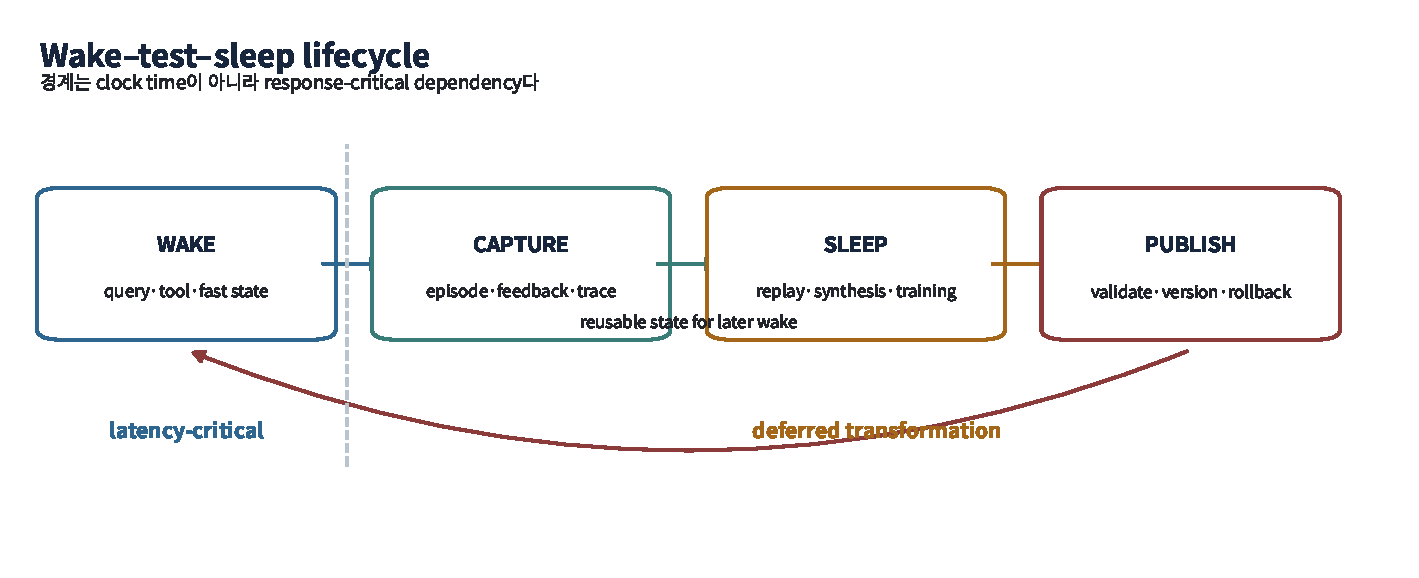
\includegraphics[width=0.98\textwidth]{figures/stc-f001.pdf}
  \caption{Wake--capture--sleep--publication의 causal lifecycle. 점선 경계 왼쪽은 현재 response의
  latency-critical path이고, 오른쪽은 후속 wake용 state를 만드는 deferred path다.}
  \stcfigure{STC-F001}
  \figsource{Original synthesis; SRC-STC-0014, SRC-STC-0052}{Wake, capture, sleep, publish 네 상자가 순서대로 연결되고 검증된 재사용 상태가 다음 wake로 되돌아오는 순환도.}
  \label{fig:stc-lifecycle}
\end{figure}

\section{Timing과 medium은 직교한다}

Update timing과 memory medium은 독립 축이다. Sleep phase는 weights, adapters, recurrent state,
text/vector store, temporal graph 또는 mixture를 바꿀 수 있다.\claim{STC-C006} 따라서 ``weights를
바꾸지 않으면 training이 아니므로 sleep도 아니다''와 ``background에서 실행되면 모두 sleep이다''는
둘 다 너무 좁거나 넓다.

\begin{figure}[htbp]
  \centering
  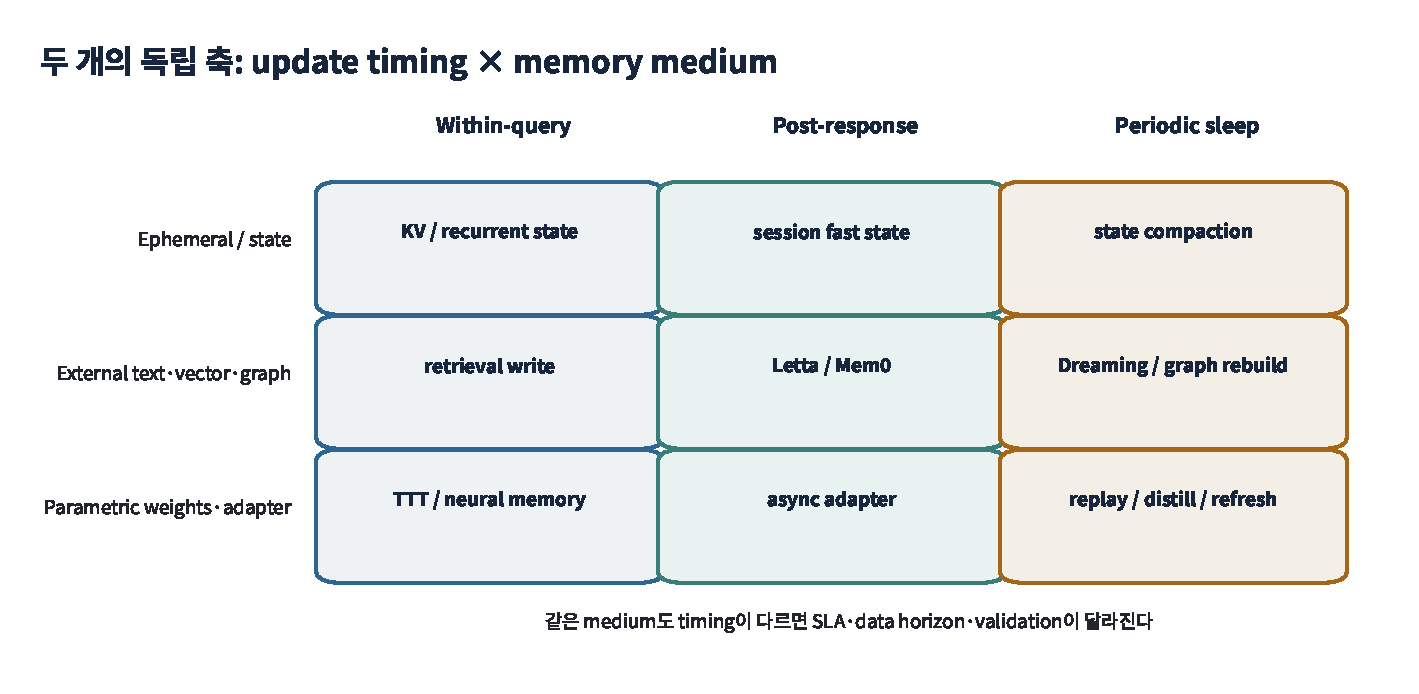
\includegraphics[width=0.98\textwidth]{figures/stc-f002.pdf}
  \caption{Update timing과 memory medium의 3$\times$3 taxonomy. 같은 LoRA update도 current answer 전에
  수행하면 test-time training, response 뒤에 수행하면 asynchronous consolidation이다.}
  \stcfigure{STC-F002}
  \figsource{Original synthesis; SRC-STC-0014, SRC-STC-0021, SRC-STC-0016}{열은 query 내부, response 이후, 주기적 sleep이고 행은 ephemeral state, 외부 text-vector-graph, parametric weight-adapter인 격자.}
  \label{fig:stc-taxonomy}
\end{figure}

분류를 위해 각 operator를 6-tuple로 기록한다.

\begin{equation}
O=(t_{trigger}, D_{horizon}, M_{source}, M_{dest}, S_{scope}, P_{publish}),
\end{equation}

여기서 trigger는 언제 시작하는지, $D_{horizon}$은 어느 기간 data를 보는지, source/destination medium은
무엇인지, scope는 query/session/user/cohort/global 중 어디인지, publication policy는 어떻게 후보를
활성화하는지 나타낸다. 같은 architecture라도 이 tuple이 다르면 system workload가 다르다.

\section{포함과 제외}

\begin{table}[htbp]
\centering
\caption{본 연구의 포함·제외 판정}
\label{tab:stc-inclusion}
\small
\begin{tabularx}{\textwidth}{p{0.27\textwidth} X X}
\toprule
행동 & 판정 & 이유 \\
\midrule
현재 query의 long chain-of-thought & 제외 & persistent reusable state를 바꾸지 않음 \\
token-by-token TTT 후 현재 답 생성 & wake/test-time & 현재 response dependency 안에 있음 \\
post-response memory agent가 profile 수정 & 포함 & deferred transformation + later reuse \\
nightly vector re-embedding/index rebuild & 포함 & external reusable state 변환 \\
LRU가 cache line을 passive eviction & 제외 & learned/validated consolidation이 아님 \\
주기적 global continued pre-training & 조건부 포함 & wake-derived stream과 explicit later-use lifecycle이면 포함 \\
배포 전 generic offline training & 제외 & wake experience와 persistent deployed loop가 없음 \\
검증 없는 background summary append & 미완성 & transformation은 있지만 publication/gate가 부재 \\
\bottomrule
\end{tabularx}
\end{table}

\section{Sleep phase와 biological stages}

NREM/REM은 replay와 perturbation, integration과 abstraction을 생각하게 하는 productive analogy다.
그러나 구현은 EEG stage를 모방할 필요가 없다. 본 연구는 기능을 다음처럼 매핑한다.

\begin{itemize}
  \item NREM-like: high-fidelity replay, recent episode integration, stable fact linking,
  \item REM-like: perturbed/generative replay, abstraction, counterfactual strategy discovery,
  \item publication: biological analogy에는 약하지만 production system에는 필수인 validation·rollback.
\end{itemize}

마지막 항이 중요한 이유는 agent memory가 사용자 data와 serving artifact를 다루기 때문이다. Biology는
배울 mechanism을 제공하지만 tenant scope, deletion SLA, source license, atomic rollout을 해결하지 않는다.

\begin{cautionbox}[Phase와 mechanism을 혼동하지 말 것]
Sleep은 \emph{언제와 어떤 lifecycle에서} 변환하는지, replay·distillation·RL·editing은 \emph{어떻게}
변환하는지, weights/text/vector/graph는 \emph{어디에} 저장하는지를 답한다. 세 질문을 분리해야
동일 resource에서 matched baseline을 만들 수 있다.
\end{cautionbox}

\chapter{Training prerequisite map: 무엇이 실제로 바뀌는가}
\label{STC-S03}

Sleep-time compute를 평가하려면 ``learning''을 하나의 동사로 쓰지 않고 data, objective, trainable
state, optimizer, validation, serving artifact로 분해해야 한다. 이 장은 별도 Training Background와
Study 사이의 navigation layer다.

\section{첫 용어 지도}

\begin{table}[htbp]
\centering
\caption{Study에서 반복 사용할 training 개념과 Background 링크}
\label{tab:study-training-map}
\small
\begin{tabularx}{\textwidth}{p{0.23\textwidth} X X}
\toprule
개념 & 최소 의미 & STC에서 묻는 질문 \\
\midrule
Fine-tuning\bgref{fine-tuning} / continued pre-training\bgref{continued-pretraining} & 좁은 목적 또는 추가 corpus로 배포 모델을 갱신 & base 전체인가, delta인가? \\
LoRA\bgref{lora} / adapter\bgref{adapter} & 작은 trainable state로 behavior를 조정 & user/domain별 artifact 수와 merge는? \\
Distillation\bgref{distillation} & teacher behavior를 student로 압축 & tail·uncertainty·provenance가 보존되는가? \\
Replay buffer\bgref{replay-buffer} / augmentation\bgref{data-augmentation} & 과거·변형 data를 new data와 섞음 & retention과 recursive-data depth는? \\
Continual learning\bgref{continual-learning} & stream을 배우며 이전 능력을 유지 & multi-cycle forgetting과 capacity knee는? \\
RLHF/RL\bgref{rlhf} & delayed/preference signal로 policy를 조정 & model이 아니라 trigger/router를 학습할 것인가? \\
Meta-learning\bgref{meta-learning} & 빠른 adaptation이 가능하도록 학습 & user sleep inner loop가 안정적인가? \\
Test-time training\bgref{test-time-training} & test stream에서 state를 즉시 갱신 & current response path인가 deferred path인가? \\
Model editing\bgref{model-editing} / unlearning\bgref{unlearning} & 좁은 수정 또는 영향 제거 & locality, lineage, rollback 단위는? \\
\bottomrule
\end{tabularx}
\end{table}

\section{Operator record}

각 연구 방법을 다음 record로 정규화한다.

\begin{equation}
R_{op}=\{D, T, \theta_{train}, \mathcal{L}/r, U, C, V, A\},
\end{equation}

$D$는 wake-derived data와 replay, $T$는 teacher/source, $\theta_{train}$은 바뀌는 state,
$\mathcal{L}/r$은 loss 또는 reward, $U$는 update rule/optimizer, $C$는 capacity destination,
$V$는 validation slices, $A$는 published artifact와 rollback unit이다. 이 record가 비어 있으면
``모델이 기억을 공고화했다''는 설명을 system으로 환원할 수 없다.

\begin{table}[htbp]
\centering
\caption{대표 sleep operator를 training record로 펼친 예}
\label{tab:study-operator-record}
\scriptsize
\begin{tabularx}{\textwidth}{p{0.12\textwidth} p{0.13\textwidth} p{0.13\textwidth} p{0.14\textwidth} X X}
\toprule
Operator & Data/teacher & Trainable state & Objective/update & Capacity & Artifact/gate \\
\midrule
summary synthesis & episodes, LLM teacher & 없음 또는 prompt/model & fidelity, utility, compression & external text & versioned record, QA \\
temporal graph & event+time+entity & graph nodes/edges & merge, supersede, conflict & external graph & graph epoch, traversal test \\
LoRA sleep & new+replay & low-rank $A,B$ & task+retention loss, Adam & adapter bank & candidate delta, shadow \\
distillation & teacher outputs+real anchor & student/base delta & CE+KL+retention & model artifact & full release suite \\
RL controller & trajectories & controller $\phi$ & delayed utility-cost reward & policy model & constrained canary \\
model edit & fact+neighbors & localized weight delta & efficacy+locality & parametric patch & edit version, rollback \\
\bottomrule
\end{tabularx}
\end{table}

\section{Training cost는 FLOPs만이 아니다}

Full fine-tuning은 weights 외에 gradient, optimizer state, activation을 필요로 한다. LoRA는 trainable
parameter와 optimizer bytes를 줄이지만 base read, forward/backward activation, validation, version
management는 남는다. External transformation은 GPU training이 없을 수 있지만 teacher inference,
embedding, graph write, dedup, index rebuild와 evaluation을 낸다.

따라서 end-to-end sleep cost를

\begin{equation}
C_{sleep}=C_{ingest}+C_{transform}+C_{train}+C_{validate}+C_{publish}+C_{retain}
\end{equation}

로 분리한다. $C_{retain}$은 artifact가 존재하는 동안의 storage, migration, rebase, deletion debt다.
Kernel FLOPs만 비교하면 external path의 retrieval cost와 parametric path의 lifecycle cost를 서로 다른
회계 기준으로 비교하게 된다.

\section{Wake, sleep, long-term memory의 세 가지 계약}

Wake path는 response SLA와 isolation을, sleep path는 throughput·deadline·candidate safety를, long-term
memory plane은 persistence·scope·version·delete를 계약한다. 한 cluster에서 모두 실행할 수도 있지만
logical contract는 분리한다. Shared state는 explicit snapshot epoch를 가져야 wake가 training 중간값을
읽지 않는다.

\begin{keypoint}[논문을 읽는 최소 checklist]
Data는 어디서 왔는가? 어느 state가 얼마나 오래 바뀌는가? Old/new/safety를 무엇으로 검증했는가?
Capacity가 찰 때 무슨 state를 제거하는가? 후보와 serving state를 어떻게 전환하는가? 이 다섯 답이
없으면 accuracy gain을 production sleep system으로 해석하지 않는다.
\end{keypoint}

\chapter{문제 분해: Sleep은 무엇을 이기려는가}
\label{STC-S04}

새 축의 가치는 이름이 아니라 기존 방법이 남긴 residual problem에서 나온다. 이 장은 sleep-time
compute가 겨냥하는 열 가지 문제를 strongest current default와 함께 놓는다.

\begin{figure}[htbp]
  \centering
  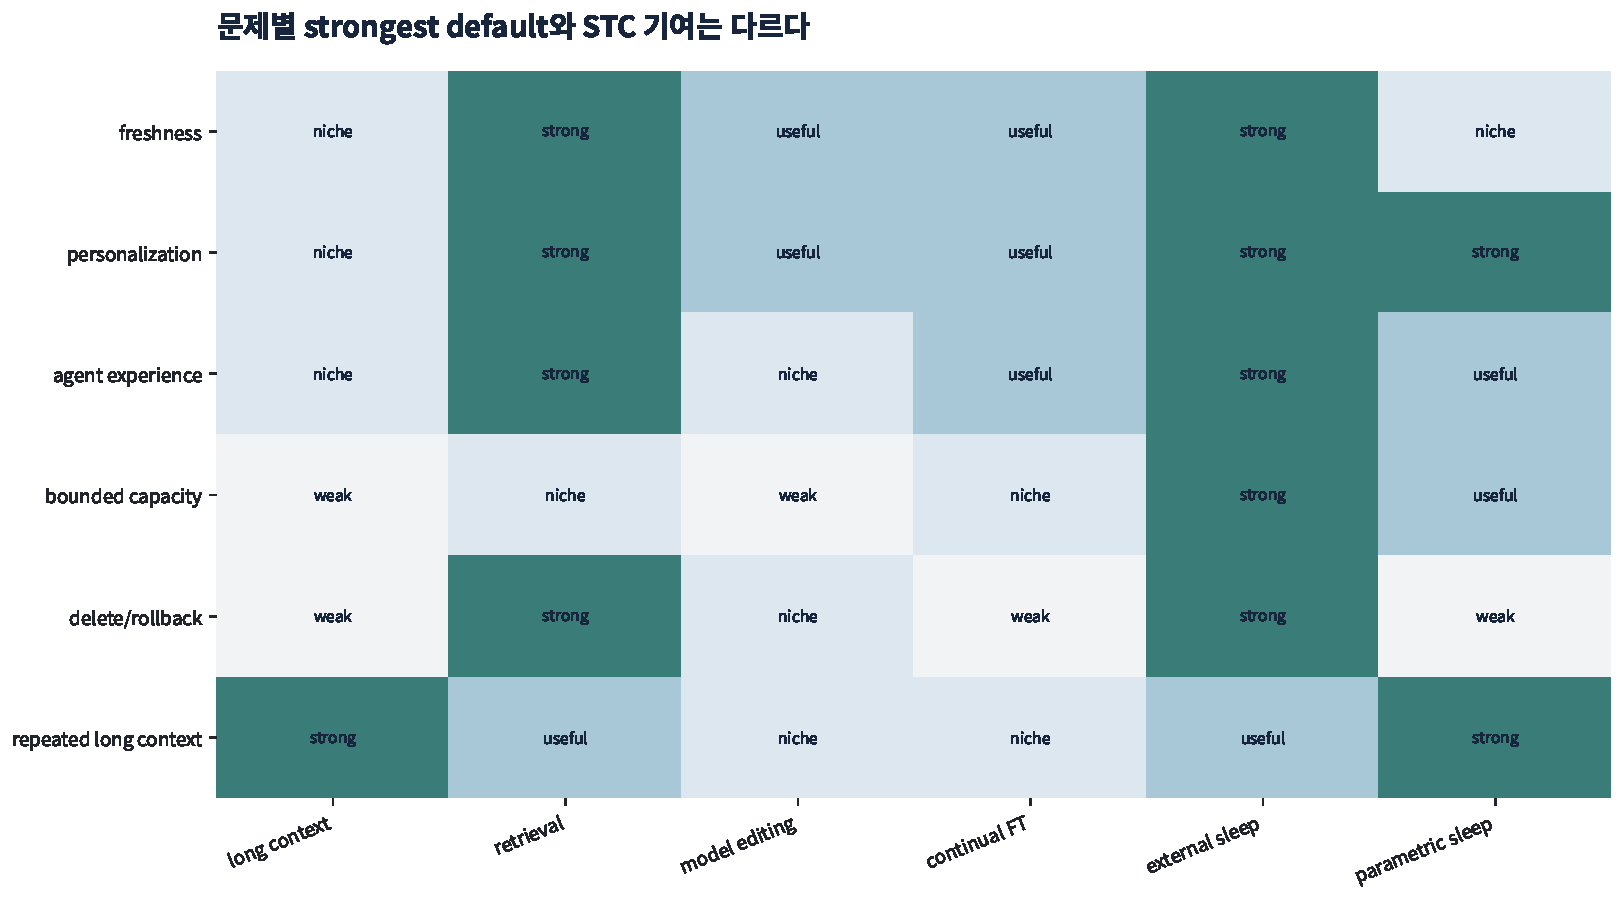
\includegraphics[width=0.96\textwidth]{figures/stc-f004.pdf}
  \caption{문제별 방법 적합도. 한 method가 모든 row에서 우세하지 않으며, external sleep과 parametric
  sleep도 서로 다른 failure surface를 가진다.}
  \stcfigure{STC-F004}
  \figsource{Original synthesis; SRC-STC-0002, SRC-STC-0031, SRC-STC-0036}{행은 freshness, personalization, agent experience, bounded capacity, deletion, repeated long context이고 열은 long context, retrieval, editing, continual FT, external sleep, parametric sleep인 색상 행렬.}
  \label{fig:problem-solution-matrix}
\end{figure}

\section{P1–P4: static deployment, personalization, experience, freshness}

\textbf{Static deployment.} Pre/post-training이 끝난 fixed model은 배포 뒤 새 사용자 분포와 도구 변화에
자동 적응하지 않는다. Strongest default는 prompt/profile retrieval과 주기적 global refresh다.
Sleep은 반복되는 local distribution을 idle window에서 정리해 다음 query의 retrieval 또는 adapter를
미리 만드는 데 기여한다. One-off interaction이면 amortization이 없다.

\textbf{Personalization.} External profile은 explicit, editable, portable하므로 첫 baseline이다. Parametric
sleep은 같은 preference가 매우 자주 재사용되고 prompt token·retrieval latency가 누적될 때 후보가 된다.
다른 user로의 leakage와 preference drift가 크면 isolated external record가 우세하다.

\textbf{Agent experience.} Agent는 성공·실패 trace에서 strategy를 추출할 수 있다. Raw transcript를
매번 long context로 넣는 대신 external strategy bank나 procedural graph로 압축하는 것이 강한 default다.
Skill이 stable하고 반복되면 distillation이나 adapter promotion을 비교한다.

\textbf{Knowledge freshness.} Mutable fact는 timestamp, supersession, citation이 필요한 external temporal
memory가 기본이다. Weight refresh는 stale fact를 지우기 어렵고 old/new fact가 composition에서 충돌할
수 있다. 실제로 sequential fact가 weights에 encoding되어도 behaviorally unreachable할 수 있으므로
retention은 parameter storage가 아니라 access와 composition으로 측정해야 한다.\claim{STC-C032}
\parencite{srcstc0036}

\section{P5–P6: continual learning과 bounded capacity}

Continual learning은 replay, regularization, gradient constraint, isolation, growth/compaction의 도움을
받지만 어느 것도 무한 retention을 보장하지 않는다. Stable skill/procedure에는 parametric integration이
유망하고, exact changing fact와 legal delete 대상에는 external representation이 유리하다.

정적 memorization capacity 실험은 sequential access, interference, governance를 포함하지 않으므로
safe continual-learning capacity를 직접 결정하지 못한다.\claim{STC-C033} \parencite{srcstc0034,srcstc0036}
Capacity는 weights의 bits뿐 아니라 replay bytes, adapter count, router fragmentation, validation time,
index latency, rollback versions의 vector budget이다.

Rate--distortion은 무엇을 어느 fidelity로 압축할지 utility--budget trade-off로 만드는 유용한 관점이지만,
제안된 frontier가 아직 agent의 보편 empirical scaling law는 아니다.\claim{STC-C034}
\parencite{srcstc0035} Future-query distortion을 reconstruction error 하나로 대체하지 말고 task utility,
provenance recovery, temporal correctness, delete granularity를 포함한다.

\section{P7–P8: latency isolation, deletion과 rollback}

Sleep의 가장 강한 system-level 이유는 expensive transformation을 current response SLA에서 분리하는
것이다. 그렇다고 반드시 별도 datacenter cluster가 필요한 것은 아니다. State가 있는 device/region에서
local sleep을 실행하면 migration을 줄일 수 있고, shared accelerator pool이 작은 job을 batch할 수도 있다.

Deletion은 source episode가 어떤 summary, vector, graph edge, training dataset, adapter에 기여했는지
lineage를 요구한다. External memory는 더 직접적이지만 poisoned record가 agent behavior를 조용히
조종할 수 있는 attack surface를 만든다. 따라서 provenance와 revocation은 부가 metadata가 아니라
설계 요구다.\claim{STC-C037} \parencite{srcstc0042}

\section{P9–P10: repeated long context와 on-device adaptation}

Long context는 원문에 대한 one-off deep reasoning에서 강하다. Sleep compilation은 context를 summary,
graph, latent/parametric state로 바꾸는 선행 비용이 있으므로 future query distribution이 예측 가능하고
reuse가 충분할 때만 이긴다. Long context를 대체하기보다 build path로 사용하고 compact state를 serve
path에서 쓰는 complement다.

On-device sleep은 privacy, intermittent connectivity, local personalization에서 expected value가 높지만
thermal, battery, write endurance, limited validation compute가 제약이다. Cloud와 device 사이에서 raw
episode 대신 provenance-preserving delta, gradient sketch, summary만 이동시키는 split도 비교 대상이다.

\section{Synthetic replay가 문제를 증폭할 때}

Generated replay를 costless fresh data로 볼 수 없다. Real-data support가 사라진 recursive training은
distribution tail을 collapse시킬 수 있다.\claim{STC-C035} \parencite{srcstc0041} 반대로 real과 synthetic
data를 적절히 누적한 조건에서 collapse는 필연이 아니므로, 중요한 변수는 synthetic 여부의 이분법보다
recursive depth와 real-data anchoring이다.\claim{STC-C036} \parencite{srcstc0069}

\begin{table}[htbp]
\centering
\caption{문제별 가장 먼저 이겨야 할 baseline과 STC의 제한된 win condition}
\label{tab:problem-baselines-short}
\small
\begin{tabularx}{\textwidth}{p{0.20\textwidth} p{0.28\textwidth} X}
\toprule
문제 & Strongest default & STC win condition \\
\midrule
freshness & temporal retrieval & 반복 query와 controlled synthesis \\
personalization & external profile & stable high reuse, reversible scope \\
agent experience & strategy memory/reflection & multi-episode compression improves later utility \\
continual skill & replay/PEFT/global refresh & cycle-level retention at bounded state \\
capacity & admit/evict/compress & marginal utility exceeds compaction/deletion cost \\
long context & long-context inference/RAG & compile cost amortized over valid reuses \\
deletion & external lineage + rebuild & parametric state remains reconstructable cache \\
\bottomrule
\end{tabularx}
\end{table}

\chapter{계보: biological replay에서 multi-rate neural memory까지}
\label{STC-S05}

Sleep-time compute는 2026년에 갑자기 생긴 단일 논문 계열이 아니다. Fast/slow learning theory,
continual learning, generative replay, external agent memory, test-time neural memory, asynchronous
memory agents가 서로 다른 문제를 풀다가 하나의 lifecycle로 수렴한다.

\begin{figure}[htbp]
  \centering
  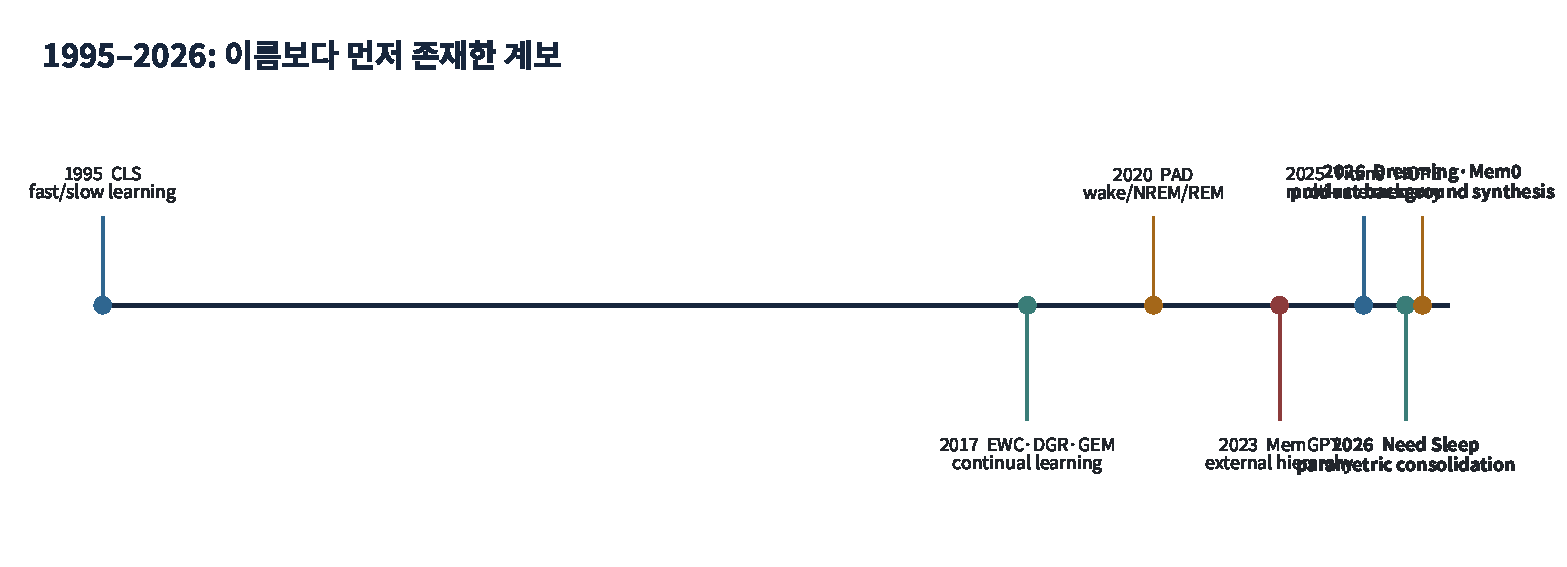
\includegraphics[width=0.98\textwidth]{figures/stc-f003.pdf}
  \caption{1995–2026 evidence chronology. 연도는 공개 source의 최초 publication/release 기준이며,
  같은 시기의 방법이 동일 maturity라는 뜻은 아니다.}
  \stcfigure{STC-F003}
  \figsource{Original synthesis; SRC-STC-0001--SRC-STC-0063}{1995 CLS에서 2017 continual learning, 2020 PAD, 2023 MemGPT, 2025 Titans/HOPE, 2026 parametric sleep과 product dreaming으로 이어지는 시간축.}
  \label{fig:stc-chronology}
\end{figure}

\section{1995: complementary learning systems}

CLS는 hippocampus의 빠른 episodic acquisition과 neocortex의 느린 interleaved learning을 분리했다
\parencite{srcstc0001}. 이 관점이 제공하는 basis는 ``새 기억을 빠르게 받는 store''와 ``기존 구조를
보존하며 천천히 통합하는 learner''를 한 update rule로 강제하지 않는다는 점이다. 오늘의 system으로
번역하면 wake log/episodic memory와 sleep consolidation model의 역할 분리다.

그러나 biology에서 production architecture를 곧바로 도출할 수는 없다. Biological model은 user
scope, exact delete, source attribution, model release compatibility를 다루지 않는다. 따라서 계보는
mechanism inspiration이지 deployment evidence가 아니다.

\section{2017: continual-learning baselines가 먼저 만든 consolidation 문제}

Deep Generative Replay는 generator의 pseudo-data와 새 data를 함께 학습해 과거 task forgetting을 줄이는
강한 non-sleep-named baseline이다.\claim{STC-C019} \parencite{srcstc0003} EWC는 이전 task에 중요한
parameter를 Fisher-weighted quadratic penalty로 보호해 stability와 plasticity를 trade-off한다.
\claim{STC-C020} \parencite{srcstc0002} GEM은 stored examples의 gradient를 constraint로 사용해 이전
task loss가 국소적으로 증가하지 않게 update를 투영한다.\claim{STC-C021} \parencite{srcstc0004}

Progress \& Compress는 active column에서 새 task를 배우고 consolidation phase에서 knowledge base로
압축하는 periodic-refresh 대안을 제시했다.\claim{STC-C022} \parencite{srcstc0007} 이 계열은 중요한
교훈을 준다. ``Sleep''이라는 이름 없이도 progress/online phase와 compress/offline phase를 나눌 수
있으며, 새 term의 가치는 matched resource에서 기존 periodic consolidation보다 나아야 한다.

\section{2020–2022: NREM/REM analogy를 계산 mechanism으로 만든 연구}

PAD(Perturbed and Adversarial Dreaming)는 wake, NREM-like perturbed replay, REM-like adversarial dreaming을
분리해 cortical representation learning을 연구했다.\claim{STC-C018} \parencite{srcstc0009}
Hippocampus--neocortex computational model은 autonomous offline dynamics와 alternating NREM/REM regime로
새 정보 통합과 old knowledge 보호를 함께 탐구했다.\claim{STC-C017} \parencite{srcstc0010}

2022년 PLOS Computational Biology의 spiking-network 연구는 두 task 설정에서 interleaved sleep-like
replay가 joint synaptic representation을 형성하고 catastrophic forgetting을 줄였다고 보고했다.
\claim{STC-C016} \parencite{srcstc0011} 이것은 user-scale LLM deployment 증거가 아니라, online data 없이
autonomous replay가 consolidation을 도울 수 있다는 mechanism evidence다. Task 수, modality, network
scale, governance의 외삽을 분리해야 한다.

\section{2023–2025: external hierarchy와 wake-time neural memory}

MemGPT는 제한된 context와 external storage 사이에서 information을 paging하는 OS-style hierarchy로
long-term agent memory를 framing했다.\claim{STC-C011} \parencite{srcstc0013} 여기서 중요한 변화는
``모델이 모든 것을 weights에 기억해야 한다''에서 ``virtual memory처럼 context와 archival memory를
관리한다''로의 이동이다.

Titans는 surprise-driven update로 test time에 neural memory state를 학습하지만, 그 자체는 wake-path
fast-state learning이지 deferred cross-session sleep은 아니다.\claim{STC-C023}
\parencite{srcstc0017} 이 구분은 user framing의 핵심이다. Test-time learning은 current/near-current
stream에 적응하고, sleep-time learning은 더 넓은 replay와 검증을 거쳐 longer-lived state를 publish한다.

Nested Learning/HOPE는 optimization process를 여러 update frequency의 nested memory level로 보아
cadence를 분석하는 유용한 틀을 제공하지만, 공개 evidence는 deployed asynchronous sleep consolidation을
입증하지 않는다.\claim{STC-C024} \parencite{srcstc0020} HOPE의 CMS처럼 서로 다른 frequency로 갱신되는
state는 wake/sleep scheduler에 자연스럽게 매핑되지만, frequency hierarchy와 lifecycle publication은
별개 요구다.

\section{2026: 명시적 parametric sleep과 product synthesis의 분기}

2026년 계보는 둘로 갈라진다. 한쪽은 Language Models Need Sleep처럼 self-modification과 replay-like
training으로 parametric memory를 통합하는 연구다. 다른 쪽은 Dreaming, Mem0 Dream, Letta처럼 external
memory를 background에서 합성하는 product lifecycle이다. 두 방향은 같은 sleep boundary를 공유하지만
state medium과 evidence maturity가 다르다.

\begin{table}[htbp]
\centering
\caption{계보별 evidence가 실제로 지지하는 범위}
\label{tab:lineage-boundaries}
\small
\begin{tabularx}{\textwidth}{p{0.20\textwidth} X X}
\toprule
계보 & 지지하는 것 & 아직 지지하지 않는 것 \\
\midrule
biological/computational sleep & autonomous replay와 multi-phase integration 가능성 & LLM fleet economics, delete/rollback \\
continual learning & forgetting을 줄이는 replay·constraint·isolation mechanism & 무한 capacity, task-free production stability \\
external agent memory & bounded context 밖 persistent state와 hierarchy & parametric skill acquisition \\
neural/test-time memory & forward path에서 learned state update 가능성 & deferred multi-session publication \\
explicit parametric sleep & self-modification+consolidation research proof & broad per-user production deployment \\
product dreaming & scheduled external background synthesis & foundation-weight training 공개 증거 \\
\bottomrule
\end{tabularx}
\end{table}

\begin{keypoint}[계보의 종합]
새로운 것은 replay 자체가 아니라, persistent agent product가 wake-derived state를 background에서 계속
변환하며 serving lifecycle로 운영하기 시작했다는 점이다. 과학적 novelty는 matched alternative 대비
효과와 scaling surface에서, 산업적 novelty는 publication·rollback·memory plane의 지속 운영에서 평가한다.
\end{keypoint}

\chapter{Alternative frontier: Sleep이 없어도 가능한 최신 경로}
\label{STC-S06}

Sleep-time compute을 promising하다고 판단하려면 이미 강한 방법을 약하게 묘사하면 안 된다. 이 장은
long context, retrieval, model editing, PEFT, context compilation, self-adaptation, recurrent memory
caching을 independent alternative 또는 component로 평가한다.

\section{Long context와 retrieval}

Long context는 원문을 손실 없이 한 번에 읽어야 하는 task의 default다. Context window와 attention
효율이 개선되면 sleep compilation의 일부 필요가 줄어든다. 그러나 매 query마다 같은 long history를
읽으면 token·KV·prefill cost가 반복되고, context selection과 stale conflict가 남는다. Sleep은 repeated
workload에서 hierarchy/summary/index를 만드는 build-time complement다.

Retrieval-Augmented Generation은 mutable knowledge를 weights 밖에 두고 retrieved passage로 generation을
condition하므로 update cost와 governance의 강한 baseline이다.\claim{STC-C026}
\parencite{srcstc0031} Record-level source, time, delete가 중요한 fact에서는 parametric sleep이 retrieval을
이기기 전에 정확도뿐 아니라 rollback과 rebase cost까지 이겨야 한다.

\section{Recurrent/neural memory와 serving cache}

RNN-style 또는 neural-memory model은 fixed-size state로 long history를 압축해 attention의 context cost를
낮출 수 있다. 그러나 prefix KV cache처럼 많은 request가 같은 reusable state를 공유하려면 state를
materialize하고 key를 정하며 cache/evict/share해야 한다. Memory Caching은 이 serving 문제를 명시한다.
\claim{STC-C025} \parencite{srcstc0022}

이는 sleep과 보완적이다. Wake model이 만드는 recurrent state를 session boundary에서 저장하고, sleep이
state를 compact/merge/rekey할 수 있다. 반대로 state reuse가 낮고 매 session이 unique하면 cache tier가
추가 complexity만 만든다. 평가에는 cache hit, state bytes, recompute cost, compatibility hash가 필요하다.

\section{PEFT: 작은 parametric destination}

LoRA는 adaptation을 low-rank weight delta로 제한해 trainable parameter와 optimizer-state cost를 줄이지만,
sequential interference와 lifecycle governance를 없애지는 않는다.\claim{STC-C027}
\parencite{srcstc0030,srcstc0036} User별 adapter가 작아도 수억 개가 되면 metadata lookup, base-version
compatibility, batching fragmentation, merge/delete가 새 serving problem이다.

PEFT는 broad full-weight sleep보다 유망한 parametric destination이다. Base를 immutable하게 두고 candidate
adapter를 version/disable하기 쉬우며, high-reuse behavior를 external profile보다 적은 wake overhead로
serve할 수 있다. 하지만 stable fact를 adapter에 넣으면 provenance와 temporal update가 어려워진다.

\section{Model editing: 좁은 update}

ROME은 transformer MLP의 factual association을 localized edit하여 targeted parametric change가 가능함을
보였지만 stable unbounded continual accumulation을 입증한 것은 아니다.\claim{STC-C028}
\parencite{srcstc0032} MEMIT은 많은 memories에 대한 mass editing을 확장했지만, 여전히 bounded batch
intervention이지 lifelong sleep loop의 증거는 아니다.\claim{STC-C029} \parencite{srcstc0033}

Editing은 correction latency가 중요하고 edit set이 작을 때 strong baseline이다. Sleep replay는 여러
episode에서 stable pattern을 통합할 때 strong하다. 양쪽 모두 efficacy 외에 paraphrase, locality, old edit
retention, multi-hop composition, rollback을 측정해야 한다.

\section{Context compilation과 one-forward adaptation}

Generative Adapter는 context를 한 forward pass로 parameter-like adapter에 compile하는 latent-memory 경로를
보인다. 그 가치는 이후 reuse가 compilation과 version management cost를 상각할 때 생긴다.
\claim{STC-C030} \parencite{srcstc0027} Gradient-based sleep보다 빠를 수 있으나 teacher/compiler quality,
base-version drift, adapter capacity, delete lineage가 남는다.

이 접근은 long context와 parametric memory의 중간점이다. 원문을 build path에서 한 번 읽고 compact
state로 serve한다. One-off document에는 compile하지 않고, predicted query count가 break-even을 넘는
document/user cluster만 선택하는 policy가 필요하다.

\section{Self-adaptation과 synthetic-data 위험}

Self-Adapting Language Models는 model이 adaptation data와 update rule을 스스로 생성해 wake learning과
later consolidation을 잇지만 recursive data quality risk를 만든다.\claim{STC-C031}
\parencite{srcstc0029,srcstc0041} Self-generated curriculum이 novelty를 늘리는지, 같은 error를 증폭하는지,
real evidence와 얼마나 연결되는지 cycle depth별로 평가한다.

\begin{table}[htbp]
\centering
\caption{Alternative frontier의 cost·capacity·governance 비교}
\label{tab:alternative-frontier}
\scriptsize
\begin{tabularx}{\textwidth}{p{0.14\textwidth} p{0.15\textwidth} p{0.15\textwidth} p{0.17\textwidth} X}
\toprule
방법 & One-time cost & Per-query cost & Capacity behavior & 주요 failure \\
\midrule
long context & 낮음 & token/KV/prefill 반복 & context window와 selection & distractor, latency \\
RAG/external & ingest/index & retrieval+context & independent storage growth & miss, poisoning, stale index \\
recurrent state & state build & small state forward & fixed/compressed state & state collision, low reuse \\
LoRA/adapter & training+validation & routing+delta compute & artifact bank 증가 & interference, fragmentation \\
model editing & locate/edit/test & 거의 없음 & edits 누적 & locality, composition \\
context compile & compiler inference & adapter reuse & compiled artifact 증가 & break-even, rebase \\
global refresh & large periodic train & model-only inference & release 단위 재압축 & freshness lag, high cost \\
\bottomrule
\end{tabularx}
\end{table}

\begin{keypoint}[Alternative와 STC의 관계]
Sleep은 별도 optimizer family가 아니다. Retrieval index rebuild, recurrent-state compaction, adapter
training, model editing, distillation, global refresh를 언제·어떤 data horizon에서 실행하고 어떻게
publish할지 묶는 lifecycle다. 따라서 ``STC vs RAG''보다 ``RAG-only vs background synthesis vs selective
promotion'' 같은 system configuration을 비교해야 한다.
\end{keypoint}

\chapter{STC mechanisms와 공개 system evidence}
\label{STC-S07}

이 장은 실제 system을 external synthesis, parametric consolidation, hybrid promotion으로 나누고,
공개 evidence가 무엇을 말하는지와 말하지 않는지를 분리한다.

\section{External-memory sleep: 현재 가장 성숙한 형태}

OpenAI Dreaming은 external user memory를 background에서 종합하는 production feature이며, 공개 설명은
per-user foundation-weight training을 말하지 않는다.\claim{STC-C007} \parencite{srcstc0052}
이는 memory item 수를 그대로 늘리는 대신 관계와 장기 pattern을 만들어 다음 interaction을 돕는다는
점에서 strict lifecycle 정의에 들어간다.

Mem0 Dream은 scheduled background synthesis와 provenance-preserving additive output을 제공하며,
merge와 supersede는 ingest-time operation으로 구분된다.\claim{STC-C008}
\parencite{srcstc0063,srcstc0064} 이 구분은 derived memory를 append-only lineage로 남기고 삭제/충돌
처리를 별도 operation으로 관리할 수 있게 한다.

Letta의 tagged sleeptime group은 response 뒤 asynchronous agent를 scheduling해 durable memory를 수정한다.
\claim{STC-C009} \parencite{srcstc0059} 즉 main agent와 memory agent를 분리함으로써 current response
latency와 background memory-writing policy를 decouple한다.

Zep/Graphiti는 episode, entity, relation을 temporal version으로 표현하며 per-user model-weight update가
아니다.\claim{STC-C010} \parencite{srcstc0016,srcstc0065,srcstc0066} Temporal edge와 supersession은 mutable
fact를 weights에 덮어쓰는 대신 history와 current truth를 함께 보존하는 강점을 가진다.

ReasoningBank는 experience에서 reusable reasoning strategy를 추출해 external strategy memory에 저장하며,
broad online weight consolidation이 아니다.\claim{STC-C012} \parencite{srcstc0043,srcstc0054} 이 계열은
``무엇을 기억할지''와 ``main model을 바꿀지''를 분리한다.

\section{Company evidence를 과대 해석하지 않기}

Meta의 personalized-agent와 HyperAgents 공개 연구는 feedback-conditioned behavior, program memory,
archive를 강조하지만 fleet-scale per-user foundation-weight sleep을 입증하지 않는다.
\claim{STC-C013} \parencite{srcstc0057,srcstc0058} ``personalization 연구''가 곧 ``nightly user weight
training product''라는 inference를 막기 위해 product, research prototype, benchmark를 구분한다.

Microsoft STATE-Bench는 state tracking, adaptation, efficiency를 함께 평가하는 memory benchmark이지,
sleep-training product 공개가 아니다.\claim{STC-C014} \parencite{srcstc0056,srcstc0067} Benchmark의
등장은 업계 문제의식을 보여 주지만 특정 mechanism adoption의 증거는 아니다.

\section{Parametric sleep: 직접적이지만 research-scale인 증거}

Language Models Need Sleep은 model이 self-modify하고 replay-like training으로 memory를 consolidate하는
parametric sleep의 직접 evidence다. 그러나 보고된 regime은 research-scale이며 production deployment
proof는 아니다.\claim{STC-C015} \parencite{srcstc0021}

Parametric path의 잠재 이점은 retrieval 없이 behavior/skill에 반영되고, repeated query에서 context
token과 external hop을 줄이며, procedural pattern을 distributed representation에 통합할 수 있다는 것이다.
동시에 다음 조건을 해결해야 한다.

\begin{itemize}
  \item multi-cycle old/new retention과 capacity saturation,
  \item base model release마다 adapter/state rebase,
  \item data lineage와 targeted delete/unlearning,
  \item candidate validation, fleet rollout, rollback,
  \item user isolation과 poisoned-memory defense,
  \item per-user job scheduling과 serving artifact explosion.
\end{itemize}

\section{Hybrid promotion}

External record를 authoritative evidence plane으로 유지하고 parametric state를 reconstructable serving
cache로 취급한다. Admission은 안정성, reuse, scope, evidence, deletion risk를 평가하고 promotion은
adapter/compiled state부터 시작한다. Global weights는 여러 cohort에 일반화되고 independent evidence가
충분할 때만 periodic refresh queue로 보낸다.

\begin{table}[htbp]
\centering
\caption{External, parametric, hybrid sleep의 운영 성질}
\label{tab:mechanism-properties}
\small
\begin{tabularx}{\textwidth}{p{0.20\textwidth} X X X}
\toprule
성질 & External & Parametric & Hybrid \\
\midrule
write/delete & item-level 쉬움 & diffuse, 어려움 & source는 쉬움, cache rebuild \\
provenance & explicit link & 간접/불완전 & external lineage가 기준 \\
wake cost & retrieval+context & 낮을 수 있음 & hot pattern만 절감 \\
capacity & storage/index 한도 & interference/state 한도 & tier별 budget \\
portability & model-independent 가능 & base-dependent & external portable, delta conditional \\
rollback & record/index version & artifact/model rollback & source replay로 재구성 \\
best content & changing facts, episodes & repeated stable behavior & fact+behavior mixture \\
\bottomrule
\end{tabularx}
\end{table}

\begin{cautionbox}[“기억했다”의 세 수준]
정보가 parameter에 encoding되었다고 해서 query에서 access되거나 다른 fact와 composition되는 것은 아니다.
저장(storage), 접근(access), 활용(composition)을 separate metric으로 보고, external/parametric 양쪽에 같은
task slice를 적용한다.
\end{cautionbox}

\chapter{Strongest-alternative matched comparison}
\label{STC-S08}

이 장은 ``아무 기억도 없는 fixed model''이 아니라 문제별 strongest plausible alternative와 STC를
matched total work, state, quality, governance에서 비교한다. Sleep phase의 장점이 transform algorithm
자체의 장점인지 scheduling/validation의 장점인지도 분리한다.

\section{비교 원칙}

\begin{enumerate}
  \item 같은 base model, wake trace, validation set, hardware budget을 사용한다.
  \item external index build와 parametric training의 ingest·validation·publish 비용을 모두 포함한다.
  \item per-query 비용은 같은 future query trace에서 측정하고 one-time cost와 분리한다.
  \item capacity budget을 맞추고 old/new/safety/delete slice를 여러 sleep cycle에 걸쳐 평가한다.
  \item source-of-truth, rollback, base-version change를 operational metric으로 포함한다.
\end{enumerate}

\section{문제별 matched baseline}

\begin{longtable}{p{0.16\textwidth} p{0.22\textwidth} p{0.24\textwidth} p{0.27\textwidth}}
\caption{문제별 strongest non-STC baseline과 조건부 verdict}\label{tab:matched-alternatives}\\
\toprule
Problem & Strongest baseline & STC candidate & Conditional verdict \\
\midrule
\endfirsthead
\toprule
Problem & Strongest baseline & STC candidate & Conditional verdict \\
\midrule
\endhead
\midrule\multicolumn{4}{r}{다음 쪽에 계속}\\
\endfoot
\bottomrule
\endlastfoot
one-off long document & long-context inference & compile/summarize before query & reuse 없으면 baseline 우세 \\
repeated corpus QA & RAG + cache & background index/summary/latent compile & valid query reuse가 break-even 초과 시 STC 가능 \\
mutable factual memory & temporal RAG/graph & scheduled conflict resolution & destination은 external sleep 우세 \\
stable user preference & profile retrieval & user adapter promotion & high reuse·low churn·easy rollback에서 parametric 후보 \\
rare correction & ROME/MEMIT or record edit & sleep batch edit/replay & immediate edit 우세, sleep은 multi-edit integration \\
continual skill & replay+PEFT/global refresh & per-domain consolidation & bounded state에서 retention 입증 시 후보 \\
agent strategy & reflection/ReasoningBank & multi-episode strategy synthesis & external sleep evidence가 강함 \\
serving efficiency & prefix/state cache & sleep state compaction & state reuse와 compatibility가 높을 때만 \\
global knowledge & scheduled continued PT & wake-derived global sleep queue & 이름보다 cadence·data quality 비교 \\
privacy-local adaptation & on-device profile/RAG & on-device LoRA/compaction & thermal/endurance 포함한 matched test 필요 \\
\end{longtable}

\section{Hybrid recommendation}

\begin{figure}[htbp]
  \centering
  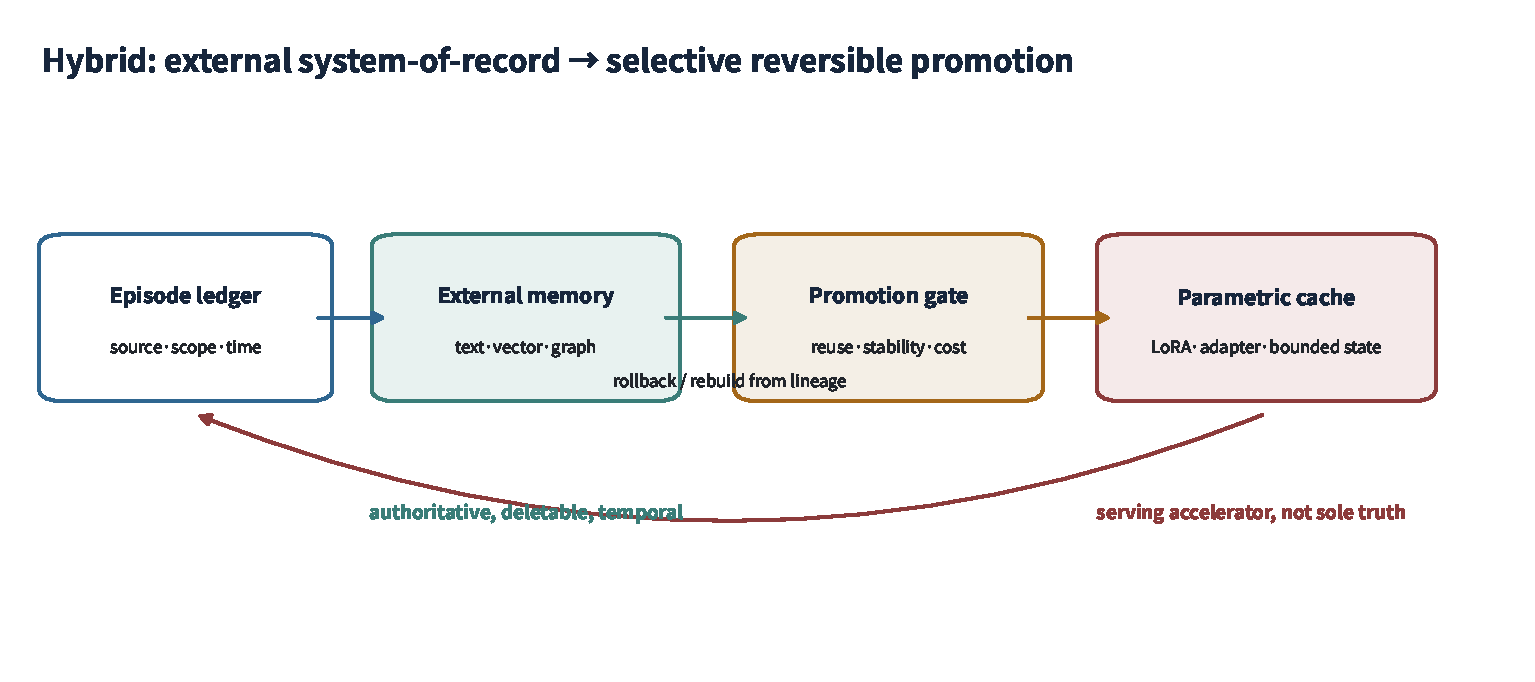
\includegraphics[width=0.98\textwidth]{figures/stc-f006.pdf}
  \caption{External system-of-record와 selective reversible parametric promotion. External evidence plane은
  authoritative하고, parametric state는 break-even을 통과한 serving cache로 취급한다.}
  \stcfigure{STC-F006}
  \figsource{Original synthesis; SRC-STC-0030, SRC-STC-0066}{Episode ledger가 external text-vector-graph memory와 promotion gate를 지나 LoRA-adapter cache로 이어지고 rollback은 provenance를 따라 원점으로 돌아가는 구조.}
  \label{fig:hybrid-promotion}
\end{figure}

Hybrid는 항상 절충안이라서 선택하는 것이 아니다. 서로 다른 content class가 요구하는 property가 다르기
때문이다. Changing fact와 rights-sensitive episode는 external source-of-record에 남고, repeated stable
behavior와 procedure는 adapter 또는 bounded neural state로 승격할 수 있다. 승격 뒤에도 original evidence를
남겨 rebase, delete, audit가 가능해야 한다.

Promotion score의 예는 다음과 같다.

\begin{equation}
P(e)=\alpha\,Reuse(e)+\beta\,Stability(e)+\gamma\,WakeSaving(e)
-\delta\,DeleteRisk(e)-\eta\,Interference(e)-\zeta\,RebaseCost(e).
\end{equation}

이는 학습된 universal score가 아니라 측정 항목을 빠뜨리지 않는 policy template다. Threshold는 user,
tenant, device, content class별로 다르며 uncertainty가 크면 external에 남긴다.

\section{STC가 이기지 못하는 영역}

\begin{itemize}
  \item 한 번만 읽는 document와 즉시 답이 필요한 query,
  \item 빠르게 변하고 exact citation·history·delete가 중요한 fact,
  \item future query distribution이 예측 불가능한 low-reuse memory,
  \item base model churn이 adapter lifetime보다 짧은 service,
  \item sleep candidate를 검증할 held-out trace가 없는 초기 product,
  \item state migration이 compute saving보다 큰 disaggregated infrastructure.
\end{itemize}

\begin{keypoint}[가장 강한 현재 판단]
External-memory sleep은 retrieval의 대체라기보다 writer·compactor·conflict resolver를 background로
옮기는 발전이다. Parametric sleep은 external system보다 본질적으로 더 긴 기억이 아니라, 반복되는
stable pattern의 serving cost를 선불로 지불하는 optimization이다.
\end{keypoint}

\IfFileExists{sections/09-evidence-trajectory.tex}{\chapter{Evidence trajectory: 무엇이 실제로 성숙하고 있는가}
\label{STC-S09}

이 장의 목적은 논문 수를 세어 momentum을 선언하는 것이 아니라, 서로 다른 종류의 증거가 어떤
주장을 허용하는지 분리하는 것이다. 연구용 알고리즘의 controlled experiment, 공개 code, 공식
product documentation, production trace, independent incident report는 같은 무게가 아니다. 또한
``sleep''이라는 단어가 없는 continual learning, external memory, state caching 연구도 lifecycle의
일부를 직접 다룰 수 있고, 반대로 생물학적 은유만 사용하는 연구는 operational STC의 증거가 아닐 수
있다.

\section{Date-frozen corpus와 재현 가능한 경계}

본 연구는 2026-08-05를 source freeze로 고정했다. Registry에는 paper, official release,
documentation, tagged repository를 합쳐 73개의 primary/official source가 들어 있다.
\claim{STC-C001} 각 source는 stable ID, canonical URL, 공개일, 접근일, source type을 가지며, 본문의
claim은 prose citation이 아니라 마지막 ledger의 exact locator로 다시 연결된다. 이 수는 검색 결과의
개수가 아니라 중복 제거와 source-kind 판정을 마친 audit surface다.

동결 시점에 명시적 background memory synthesis를 설명한 공개 production lineage는 적어도
OpenAI Dreaming과 Mem0 Dream 두 개였다.\claim{STC-C002}
\autocite{srcstc0052,srcstc0063} Letta의 tagged sleeptime code와 Zep/Graphiti의 temporal provenance는
같은 lifecycle을 다른 component에서 보강하지만, product-scale comparative effectiveness를 대신하지
않는다. 공식 release는 ``기능이 존재한다''를 지지할 수 있어도 ``strongest baseline보다 우월하다''를
지지하지 못한다.

검색은 saturation을 과장하지 않는다. 12개 cluster 중 2개만 bounded closure, 5개는 active frontier,
5개는 measurement gap으로 닫혔다.\claim{STC-C003} 특히 utility--sleep compute, utility--memory
budget, retention--update count, bytes moved--placement curve가 없는 cluster는 source가 많아도
``saturated''로 부르지 않았다. 이 규칙은 2026-08-05 이후의 발견이 결론을 바꿀 수 있음을 문서 구조에
남긴다.

\section{Evidence maturity와 expected value는 다른 축이다}

\begin{table}[htbp]
\centering
\caption{본문에서 사용하는 evidence maturity ladder}
\label{tab:evidence-ladder}
\begin{tabularx}{\textwidth}{C{0.09\textwidth} L{0.28\textwidth} Y Y}
\toprule
Level & 최소 근거 & 허용되는 문장 & 허용되지 않는 확대 해석 \\
\midrule
E0 & 아이디어·명칭 & 제안되었다 & 작동한다 \\
E1 & 단일 synthetic/offline 실험 & 제한된 setting에서 관측됐다 & 일반화된다 \\
E2 & 다중 task/model 또는 code & 조건부로 지지된다 & production-ready다 \\
E3 & strong baseline, ablation, long horizon & 평가 범위에서 경쟁력 있다 & fleet economics가 성립한다 \\
E4 & 공식 production lifecycle & 공개 제품에서 동작한다 & scientific optimum이다 \\
E5 & independent deployment trace·incident & 운영 성질이 독립 확인됐다 & 다른 workload에도 보편적이다 \\
\bottomrule
\end{tabularx}
\end{table}

Expected value가 높아도 evidence가 E1이면 high-upside research bet이다. 반대로 E5인 query-time
retrieval이 특정 high-reuse procedural workload에서 가장 값싼 해답이라는 뜻도 아니다. 본 논문은
problem severity, quality advantage, cost advantage, evidence maturity, deployment fit, governance,
industry momentum, academic momentum을 각각 기록하고 평균 점수 하나로 숨기지 않는다.

\section{Industry와 academia의 서로 다른 수렴}

\begin{figure}[htbp]
  \centering
  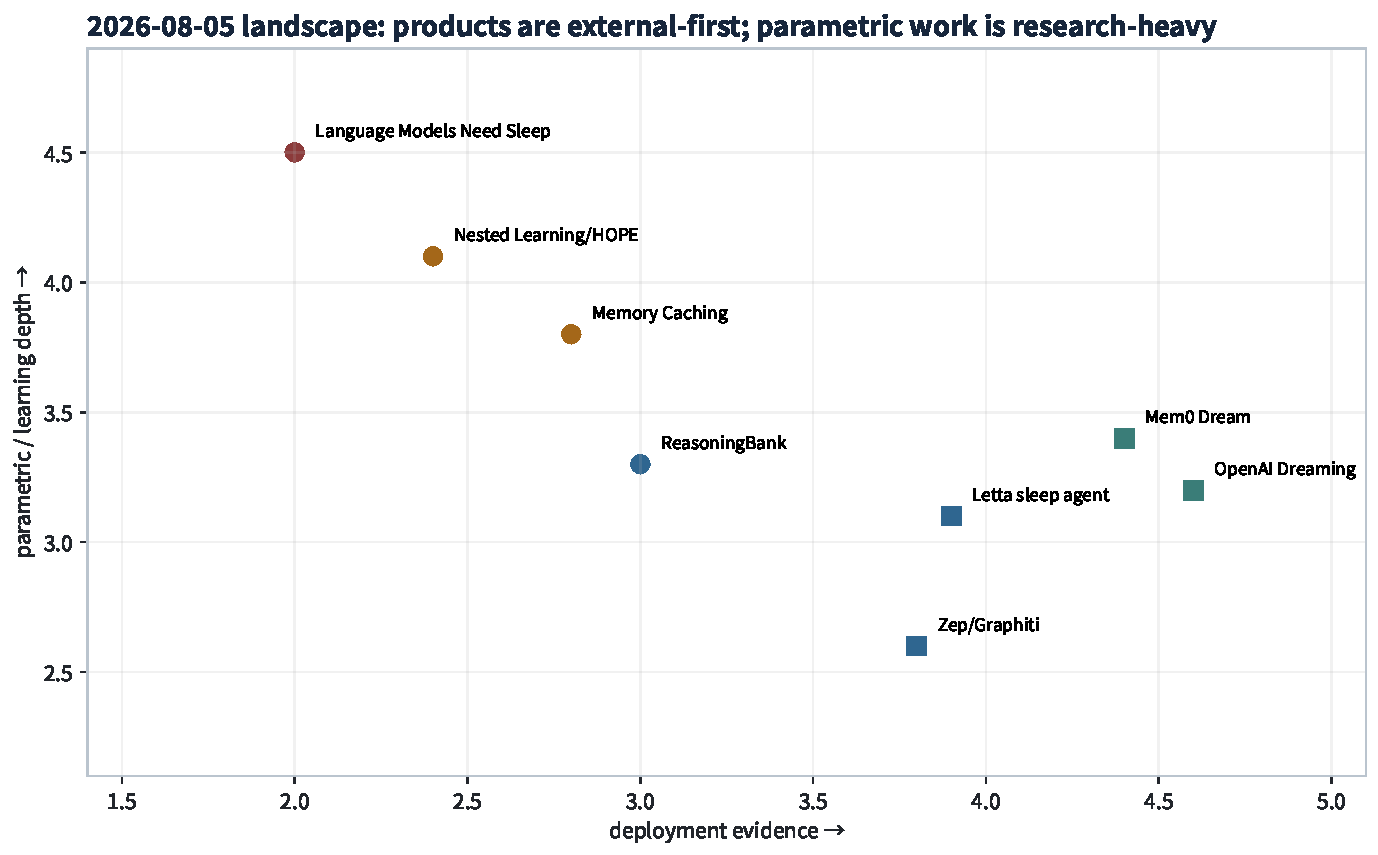
\includegraphics[width=0.96\textwidth]{figures/stc-f014.pdf}
  \caption{Source freeze 시점의 industry--academia landscape. Industry는 external synthesis와
  temporal provenance에, academia는 continual learning, neural memory, learned writer와 capacity
  theory에 더 넓게 분포한다. 좌표는 corpus의 정성적 audit를 시각화한 것이며 시장 규모가 아니다.}
  \stcfigure{STC-F014}
  \figsource{Original synthesis; SRC-STC-0054, SRC-STC-0056, SRC-STC-0057}{제품과 연구 lineages를 external lifecycle, learned memory policy, parametric consolidation, benchmark/theory 축에 배치한 지도.}
  \label{fig:industry-academia}
\end{figure}

Industry에서 가장 분명한 경로는 episode 보존 $\rightarrow$ contradiction/dedup $\rightarrow$
scheduled pattern synthesis $\rightarrow$ future retrieval $\rightarrow$ user control/provenance다.
Academia의 경로는 더 넓다. Replay와 continual-learning regularization, test-time neural memory,
memory writer/router RL, rate--distortion compaction, self-evolving strategy memory, sequential fact
reachability가 서로 다른 이름으로 같은 admission--transform--destination--validation 문제를 만든다.
\autocite{srcstc0020,srcstc0021,srcstc0035,srcstc0043,srcstc0051}

따라서 momentum에 대한 정확한 표현은 ``external background transformation은 I3/E4에 도달했고,
learned external policy는 빠른 E2--E3 frontier이며, broad per-user parametric sleep은 E1--E2''다.
이 세 문장을 하나의 ``STC가 뜬다''로 합치면 투자 방향과 실험 설계가 모두 왜곡된다.

\section{번역 corpus가 담당하는 역할}

전체 source를 모두 번역하는 대신, explicit sleep, biological/computational precursor, continual
learning, external memory, neural memory, capacity, negative evidence를 가로지르는 15편을 balanced
translation corpus로 고정했다.\claim{STC-C004} 번역본은 의견을 추가하는 secondary review가 아니라
원문의 section·figure·limitation을 보존하는 독해 보조물이다. 반면 이 Study는 그 source들을
problem과 lifecycle 기준으로 재조합하는 분석이다. 두 산출물을 분리해야 번역자의 해석이 원저자의
주장처럼 보이지 않는다.

\begin{keypoint}[Evidence trajectory의 결론]
새로운 축의 가장 강한 증거는 하나의 breakthrough paper가 아니다. Continual-learning mechanism,
external-memory product, asynchronous implementation, temporal provenance, realistic benchmark가 서로
다른 층에서 같은 lifecycle boundary를 채우기 시작했다는 점이다. 다만 parametric destination의
장기 retention·delete·rollback·fleet cost를 동시에 보여 주는 공개 증거는 아직 비어 있다.
\end{keypoint}
}{}
\IfFileExists{sections/10-promisingness.tex}{\chapter{Promisingness: 새로운 축은 정말 최선인가}
\label{STC-S10}

질문은 ``sleep이라는 이름이 흥미로운가''가 아니라, 동일한 wake evidence와 future query를 주었을 때
deferred transformation이 long context, RAG, periodic refresh, model editing, wake TTT보다 더 나은
lifetime frontier를 만드는가다. 여기서 frontier는 quality만이 아니라 total retained state, later-wake
cost, freshness, delete, rollback, wake-SLA까지 포함한다.

\section{현재 증거가 지지하는 범위}

공개 industry evidence는 external-memory sleep과 background synthesis에서 가장 강하며, 광범위한
per-user foundation-weight sleep에서는 그렇지 않다.\claim{STC-C038}
\autocite{srcstc0052,srcstc0059,srcstc0063,srcstc0065} 이는 external 방식이 영원히 우월하다는
뜻이 아니라, 이미 배포된 lifecycle과 아직 연구-scale인 parametric mechanism을 구분한다는 뜻이다.

Broad parametric sleep은 continual retention, rollback, deletion, security, fleet serving economics를
동시에 입증하지 못했다.\claim{STC-C039} ``Language Models Need Sleep''은 self-modification과
consolidation의 direct evidence지만 연구 규모의 method result이고, sequential fact learning은 weight에
남은 정보가 normal behavior에서 접근 불가능해질 수 있음을 보여 준다. External memory도 poisonable하기
때문에 단순히 외부에 두면 문제가 끝나는 것은 아니다.\autocite{srcstc0021,srcstc0036,srcstc0042}

\begin{figure}[htbp]
  \centering
  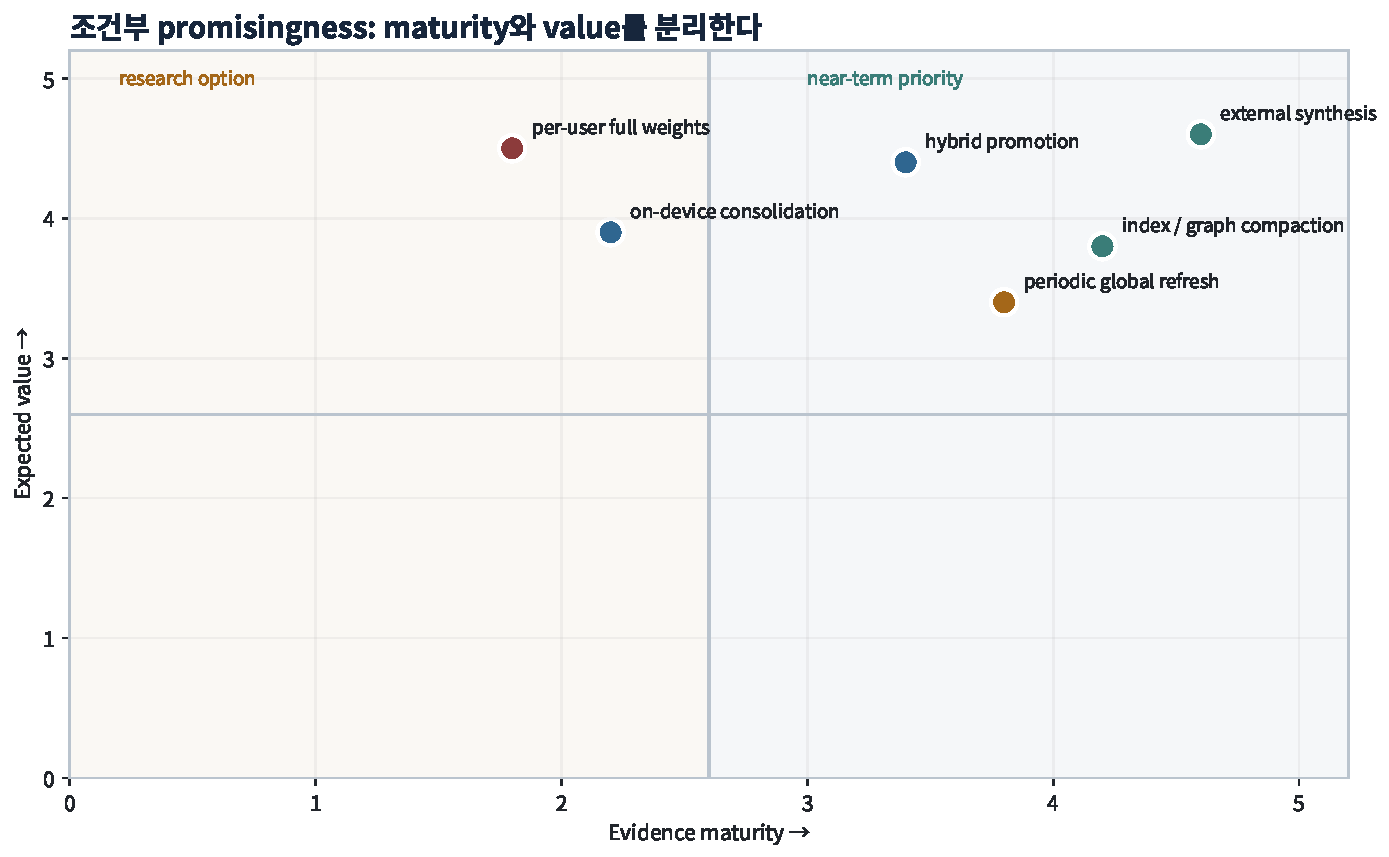
\includegraphics[width=0.96\textwidth]{figures/stc-f005.pdf}
  \caption{Evidence maturity와 expected value를 분리한 conditional verdict. 오른쪽 위로 갈수록 현재
  증거와 잠재 가치가 함께 높다. Parametric sleep은 잠재 가치가 커도 성숙도가 낮은 연구 bet로 남는다.}
  \stcfigure{STC-F005}
  \figsource{Original synthesis; SRC-STC-0052, SRC-STC-0063, SRC-STC-0021}{External synthesis, learned writer, adapter promotion, broad weight update를 성숙도와 기대 가치의 두 축에 배치한 산점도.}
  \label{fig:conditional-promisingness}
\end{figure}

가장 신뢰할 중기 구조는 auditable external system-of-record에 원 증거를 남기고, stable하고
high-reuse인 일부만 reversible adapter 또는 bounded parametric state로 승격하는 hybrid다.
\claim{STC-C040}\autocite{srcstc0027,srcstc0030,srcstc0052,srcstc0066}
Parametric artifact는 기억의 원장이 아니라 serving을 위한 compiled cache로 취급한다. Base model,
consent, evidence validity가 바뀌면 external source에서 다시 만들 수 있어야 한다.

\section{여섯 개의 핵심 verdict}

\begin{longtable}{L{0.16\textwidth} L{0.19\textwidth} L{0.28\textwidth} L{0.22\textwidth}}
\caption{핵심 주장별 조건부 verdict와 반증 조건}\label{tab:promisingness-verdicts}\\
\toprule
Claim & Verdict & 근거가 허용하는 범위 & Confidence를 낮출 관측 \\
\midrule
\endfirsthead
\toprule
Claim & Verdict & 근거가 허용하는 범위 & Confidence를 낮출 관측 \\
\midrule
\endhead
새 scaling phase인가 & functional level에서 yes & release-time training도 current-query reasoning도 아닌 durable later-wake state budget & matched synchronous maintenance와 차이가 전혀 없음 \\
mainstream인가 & lifecycle은 likely, 명칭·parametric form은 uncertain & persistent agent의 background synthesis/validation & 주요 platform이 scheduled transform을 채택하지 않음 \\
long context의 최선인가 & generally no & predictable high-reuse query에서 compile break-even 가능 & high reuse에서도 quality/cost crossover 없음 \\
continual learning 해결인가 & useful phase, solution theorem은 아님 & replay·regularization·isolation을 실행할 시간 경계 제공 & repeated cycle에서 빠른 capacity knee \\
parametric이 external보다 우월한가 & content-dependent & stable skill은 compile, volatile exact fact는 external & 단일 medium이 모든 축에서 지배 \\
device opportunity인가 & workload는 yes, 제품 claim은 별도 검토 & version, lineage, compaction, mixed read/write가 새 trace 생성 & 실제 trace가 작은 metadata job에 머묾 \\
\bottomrule
\end{longtable}

\section{문제별 strongest alternative와 sleep의 조건}

\textbf{One-off long context.} 한 번 읽고 답하는 문서는 FlashAttention 기반 long context 또는 RAG가
정확한 evidence와 citation을 보존한다. Sleep compilation은 query 전에 비용을 내고 정보 손실과
staleness를 추가하므로 reuse 예측이 없으면 열세다.

\textbf{Mutable factual memory.} Temporal graph와 versioned retrieval이 현재값, 과거값, supersession,
delete를 직접 표현한다. Parametric write가 경쟁하려면 normal-query reachability와 exact reversal을
추가로 증명해야 한다.

\textbf{Repeated procedure와 strategy.} 동일 repository, tool, enterprise procedure가 반복되면
retrieval/context token과 reasoning latency를 매번 지불한다. 이때 background synthesis, learned
strategy memory, adapter compilation이 유망하다. 다만 exact-repeat가 아니라 held-out semantic transfer로
효과를 측정해야 한다.\autocite{srcstc0043,srcstc0054}

\textbf{Global common knowledge.} 사용자별 sleep보다 centralized continued pre-training과 periodic
refresh가 더 넓게 amortize된다. STC가 이기려면 central release cadence보다 빠른 local adaptation 또는
공유할 수 없는 private evidence라는 조건이 필요하다.

\textbf{On-device personalization.} Idle window, privacy, intermittent connectivity는 sleep scheduling과
잘 맞지만 thermal, battery, write endurance, recovery state까지 포함한 측정이 없다면 가능성만 말할 수
있다. Cloud 비용을 device 비용으로 옮긴 것을 효율 향상으로 세면 안 된다.

\section{Workload별 판단}

\begin{table}[htbp]
\centering
\caption{Workload별 expected value와 현재 evidence maturity}
\label{tab:workload-promisingness}
\begin{tabularx}{\textwidth}{L{0.25\textwidth} C{0.14\textwidth} C{0.18\textwidth} Y}
\toprule
Workload & 가치 & 성숙도 & 현재 추천 \\
\midrule
multi-year personal assistant & 높음 & E4 external / E1 parametric & external synthesis 우선 \\
enterprise procedure/coding & 매우 높음 & E2--E3 & external strategy + selective adapter 실험 \\
one-off document QA & 낮음--중간 & E5 baseline & long context/RAG 우선 \\
recurring technical corpus & 높음 & E2 & reuse sweep 뒤 compile \\
universal current facts & 중간 & E5 refresh/RAG & global refresh + retrieval \\
private local adaptation & 높음 & E1 & thermal/endurance 포함 pilot \\
high-churn profile & external 높음 & E4 external & versioned external only \\
robotics/autonomy & 높음 & E1--E2 & safety-gated domain sleep \\
\bottomrule
\end{tabularx}
\end{table}

\section{의사결정 규칙}

새 evidence $e$를 destination $j$로 compile하는 decision은 단순 score가 아니라 최소 다목적 제약이다.

\begin{equation}
\text{promote}(e,j) \Longleftrightarrow
\begin{cases}
\widehat R_v(e)\,\Delta U_j(e) > C_{life}(e,j),\\
P(\text{valid at reuse}) \ge \tau_v,\\
\text{delete/rollback/compatibility gates pass},\\
\Delta U_{old},\Delta U_{safety} \ge -\epsilon.
\end{cases}
\end{equation}

하나라도 모르면 external에 남기는 것이 기본값이다. 이 규칙은 STC를 특별 대우하지 않는다. External
summary도 원본을 버리거나 false merge를 만들 수 있으므로 같은 validation과 lineage gate를 통과해야
한다.

\begin{keypoint}[Promisingness verdict]
Sleep-time compute은 하나의 universal method가 아니라 미래 wake를 위해 비용을 선불 지불하는 lifecycle
class다. 현재 가장 promising한 부분은 external background transformation과 learned memory policy이고,
가장 high-upside지만 불확실한 부분은 selective reversible parametric promotion이다. Continuous per-user
base-weight update는 현재 strongest default가 아니다.
\end{keypoint}
}{}
\IfFileExists{sections/11-mainstream-scenarios.tex}{\chapter{Mainstream scenarios: lifecycle과 이름의 미래}
\label{STC-S11}

미래를 하나의 확률 숫자로 압축하면 workload 차이를 잃는다. Consumer assistant는 external-memory
dominant이면서, enterprise coding agent는 hybrid promotion을 쓰고, foundation-model vendor는
periodic global refresh를 유지할 수 있다. 따라서 다섯 시나리오는 상호 배타적 시장 예측이 아니라
기술·경제 조건에 따른 system shape다.

더 중요한 언어적 주의가 있다. 이 lifecycle이 주류가 되어도 ``sleep-time compute''이라는 명칭이
승리할 필요는 없다. 공개 system은 dreaming, reflection, synthesis, memory, self-evolution,
consolidation이라는 서로 다른 말을 쓴다.\claim{STC-C042}
\autocite{srcstc0052,srcstc0054,srcstc0060,srcstc0063} 따라서 adoption은 keyword count가 아니라
deferred execution, wake-derived input, durable destination, later-wake reuse라는 operational signature로
추적해야 한다.

\section{다섯 개의 조건부 시나리오}

\begin{longtable}{L{0.15\textwidth} L{0.23\textwidth} L{0.25\textwidth} L{0.22\textwidth}}
\caption{시나리오별 trigger, leading indicator, falsifier}\label{tab:mainstream-scenarios}\\
\toprule
Scenario & Trigger & Leading indicators & Falsifiers \\
\midrule
\endfirsthead
\toprule
Scenario & Trigger & Leading indicators & Falsifiers \\
\midrule
\endhead
External dominant & provenance/delete 요구, frequent base upgrade, retrieval 개선 & pattern/supersede/cadence API, portable temporal memory, memory incident tooling & procedural skill을 지속적으로 잃거나 retrieval cost가 고정 병목 \\
Hybrid promotion & calibrated reuse predictor, cheap adapter validation/routing, source lineage & promote/demote/rebuild API, adapter catalog, reuse sweep benchmark & dual-state consistency와 version churn이 saving을 상쇄 \\
Periodic refresh & global amortization 우세, local history retention 제한 & release cadence 단축, central synthetic/eval factory, source-based adapter regeneration & local procedure가 release 사이에 빠르게 변함 \\
STC niche & 높은 reuse가 일부 domain에만 존재, validation cost 큼 & domain/cohort adapter, ROI/pressure trigger, repeated-task gain & general assistant에서도 background synthesis가 표준화 \\
STC broad & hundreds-cycle 안정성, bounded delete/rollback, stable queue, migration economics & wake/sleep quota와 SLO, durable state handle, lifecycle scaling curves & validation·state fan-out·privacy cost가 benefit보다 빠르게 증가 \\
\bottomrule
\end{longtable}

\section{현재 base case}

동결된 증거와 가장 일치하는 조합은 세 줄이다.

\begin{enumerate}
  \item \textbf{Near term: external-memory dominant.} Background synthesis, dedup, conflict resolution,
  temporal graph, provenance가 foundation weight를 바꾸지 않고 먼저 확산한다.
  \item \textbf{Evolution: high-reuse stable skill에서 hybrid promotion.} External source-of-record를
  버리지 않고 adapter, expert, latent cache를 제한적으로 compile한다.
  \item \textbf{Coexistence: global common knowledge는 periodic refresh.} 모든 durable learning을
  사용자별 sleep job으로 분해하지 않는다.
\end{enumerate}

STC niche의 가장 강한 형태, 즉 general assistant에는 background transformation이 거의 없을 것이라는
예측은 OpenAI와 Mem0 evidence로 이미 약해졌다. 반대로 continuous per-user parametric learning이
표준이 될 것이라는 broad scenario는 repeated-cycle E3와 production E4가 없다.

\section{분기점을 미리 보여 주는 signal}

\begin{table}[htbp]
\centering
\caption{Quarterly signal dashboard}
\label{tab:scenario-signals}
\begin{tabularx}{\textwidth}{L{0.32\textwidth} Y L{0.25\textwidth}}
\toprule
관측할 signal & 의미 & 어느 방향을 강화하는가 \\
\midrule
public per-user weight/adapter update와 rollback trace & parametric lifecycle 성숙도 & hybrid/broad \\
memory provenance·supersede·delete API 확장 & external governance maturity & external/hybrid \\
reuse predictor calibration과 top-$k$ yield & compile economics & hybrid/niche \\
base upgrade 후 adapter/index rebuild cost & artifact lifetime & refresh 대 hybrid \\
100--1,000 cycle retention/plasticity curve & lifelong claim 가능성 & broad 또는 반증 \\
background job bytes, energy, queue age & 실제 infra workload & 모든 시나리오의 device 규모 \\
learned writer/router의 cross-domain result & main-model update 대안 & external/hybrid \\
on-device idle training trace & privacy-local fit & niche/broad \\
\bottomrule
\end{tabularx}
\end{table}

\section{시나리오에 강건한 연구 전략}

예측에 베팅하기보다 공통 분모를 먼저 만든다. Immutable wake event와 lineage, versioned candidate,
validation attestation, atomic publish/rollback, total-state accounting은 external-only에서도 필요하고
hybrid와 broad adoption에서는 더 중요하다. Algorithm research는 reuse·volatility·capacity sweep으로
어떤 item을 external에 남기고 무엇을 promote할지 학습한다. Hardware research는 특정 ``sleep
accelerator'' 명칭보다 state locality, mixed rewrite, snapshot, metadata tail latency를 측정한다.

\begin{cautionbox}[Scenario를 달력 예측으로 읽지 않기]
이 장은 2028년 market share를 예측하지 않는다. 각 시나리오가 성립하려면 어떤 공개 evidence가
나타나야 하고 무엇이 confidence를 낮추는지 미리 고정한다. 새 정보가 들어오면 narrative가 아니라
trigger와 falsifier를 갱신한다.
\end{cautionbox}
}{}
\IfFileExists{sections/12-scaling-law.tex}{\chapter{Scaling law: 법칙이 아니라 측정 가능한 가설부터}
\label{STC-S12}

Pre-training scaling은 통제된 data, parameter, compute와 loss의 관계를 다룬다. STC에는 previous
state, wake evidence, admission policy, memory medium, cycle count, future query reuse, validation과
publication이 추가되어 path-dependent하다. 따라서 ``accuracy versus sleep FLOPs'' 한 곡선은 state가
증가했는지, data가 좋아졌는지, future reuse가 달랐는지 구분하지 못한다.

동결 corpus의 어느 source도 보편적인 sleep-time scaling law를 확립하지 않는다.\claim{STC-C041}
\autocite{srcstc0034,srcstc0035,srcstc0050} 아래 식은 \measured{} accounting identity,
\analytical{} break-even, \fitcandidate{}, \hypothesis{}의 네 등급으로 분리한다. 관측 전 가설을
``law''라고 부르지 않는 것이 이 장의 가장 중요한 결과다.

\begin{figure}[htbp]
  \centering
  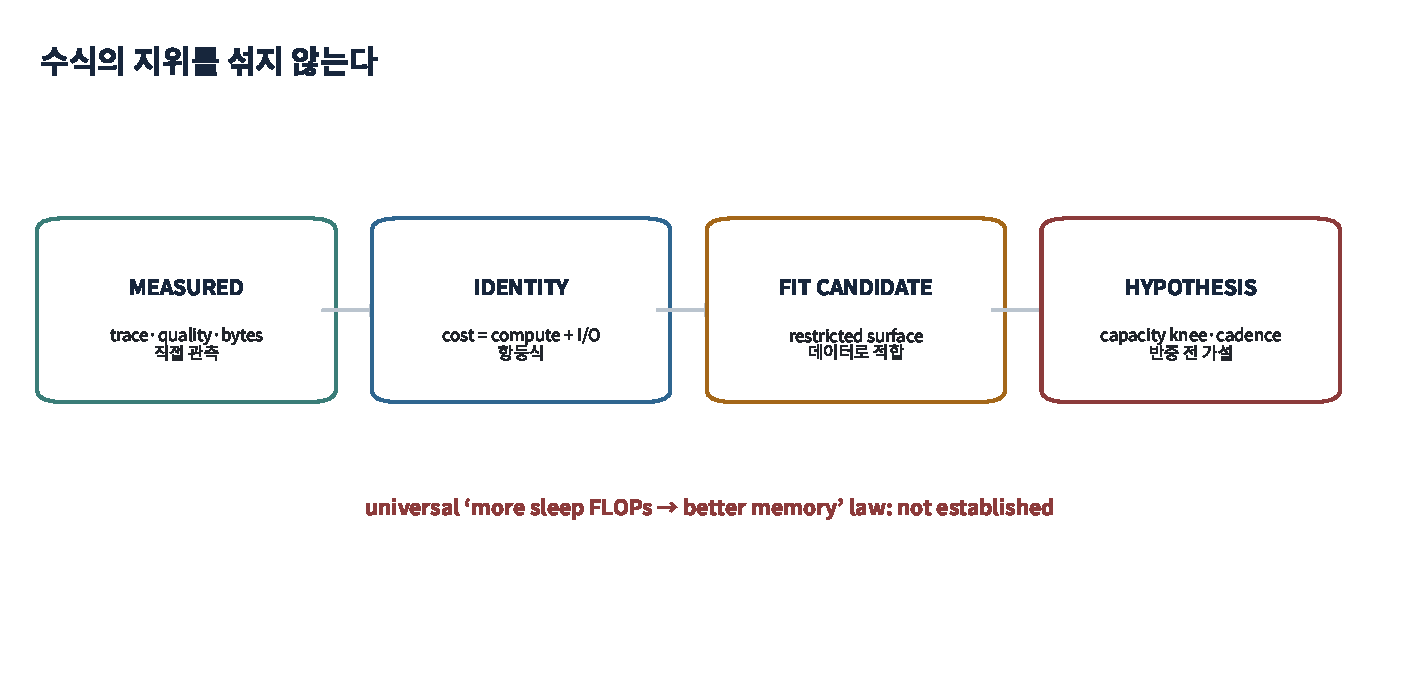
\includegraphics[width=0.98\textwidth]{figures/stc-f007.pdf}
  \caption{Scaling statement의 네 등급. Identity는 장부를 닫고, break-even은 제한된 가정 아래
  경계를 계산하며, fit candidate는 sweep에 맞추고, hypothesis는 반증 실험을 기다린다.}
  \stcfigure{STC-F007}
  \figsource{Original synthesis; SRC-STC-0035, SRC-STC-0050}{측정식에서 보편 법칙으로 갈수록 필요한 가정과 검증 범위가 증가하는 네 단계 사다리.}
  \label{fig:scaling-evidence-ladder}
\end{figure}

\section{State와 lifecycle work를 먼저 닫는 identity}

Answer-bearing retained state를 destination 하나로 축소하면 안 된다.

\begin{equation}
B_{retained}=B_r+B_e+B_l+B_p+B_a+B_v,
\label{eq:retained-state}
\end{equation}

여기서 $B_r$은 canonical/raw evidence, $B_e$는 text/vector/graph/index, $B_l$은 latent·KV·recurrent
state, $B_p$는 adapter/expert/weight delta, $B_a$는 optimizer·importance·router·teacher support,
$B_v$는 lineage·predecessor·rollback state다. Active summary bytes만 보고 ``압축률''을 계산하면 archive와
recovery copy가 사라진 것처럼 보이는 오류가 생긴다.

동시에 존재하는 candidate, pinned predecessor, migration, workspace, replica까지 더한 peak는

\begin{align}
B_{peak,state}(t)={}&B_{retained}(t)+B_{candidate}(t)+B_{pinned}(t)\nonumber\\
&+B_{migration}(t)+B_{workspace}(t)+B_{replica}(t),\\
B_{peak,physical}(t)={}&B_{base,resident}(t)+B_{peak,state}(t)+B_{execution}(t).
\end{align}

Physical maximum은 각 항의 서로 다른 시간대 high-water mark를 더하지 않고 같은 timestamp에서
평가한다. Separate wake/sleep fleet가 contention을 줄이면서 base model replica를 늘릴 수 있으므로
incremental state와 physical placement를 둘 다 보고해야 한다.

Full-history replay는 특히 위험하다. Cycle $t$에서 이전 task의 $m_i$개를 모두 replay하면

\begin{equation}
W_T=\sum_{t=1}^{T}\sum_{i=1}^{t}m_i
=\sum_{i=1}^{T}m_i(T-i+1).
\end{equation}

$m_i=m>0$이면 $W_T=mT(T+1)/2=\Theta(T^2)$다. Admission fraction을 일정 비율 줄이는 것만으로는
계수만 줄고 차수가 바뀌지 않는다. Bounded memory를 주장하려면 expire, compaction, coreset,
generated replay 또는 selective revisit가 실제로 lifetime work와 retained state를 제한하는지 보여야 한다.

\section{Valid reuse가 만드는 compile break-even}

Sleep artifact $i$의 가치에서 raw memory count나 sleep FLOPs보다 유용한 후보 변수는 valid reusable
evidence per lifecycle cost다.\claim{STC-C043}\autocite{srcstc0035,srcstc0043,srcstc0051}
그 이유는 compile이 한 번 비싸도 미래에 반복 사용되면 이득이고, 수천 개 memory를 만들었어도 다시
쓰이지 않으면 이득이 0이기 때문이다.

Stationary하고 quality가 같다는 제한된 가정에서 reuse break-even은

\begin{equation}
n^*=\frac{C_{compile}+C_{maint}}{\Delta C_{use}}.
\label{eq:reuse-break-even}
\end{equation}

Validity survival과 discount를 넣으면 horizon $H$의 expected valid reuse는

\begin{equation}
R_i(H)=\int_0^H \lambda_i(t)S_i(t)e^{-\omega t}\,dt.
\end{equation}

Promotion은 $R_i(H)\Delta U_{ij}$가 compile, serve, governance, risk cost의 합보다 클 때만 후보가 된다.
Future reuse를 oracle로 쓰지 않기 위해 실제 router는 past-only feature로 $\widehat R_i$를 예측하고,
calibration error도 lifecycle cost에 넣는다.

\begin{figure}[htbp]
  \centering
  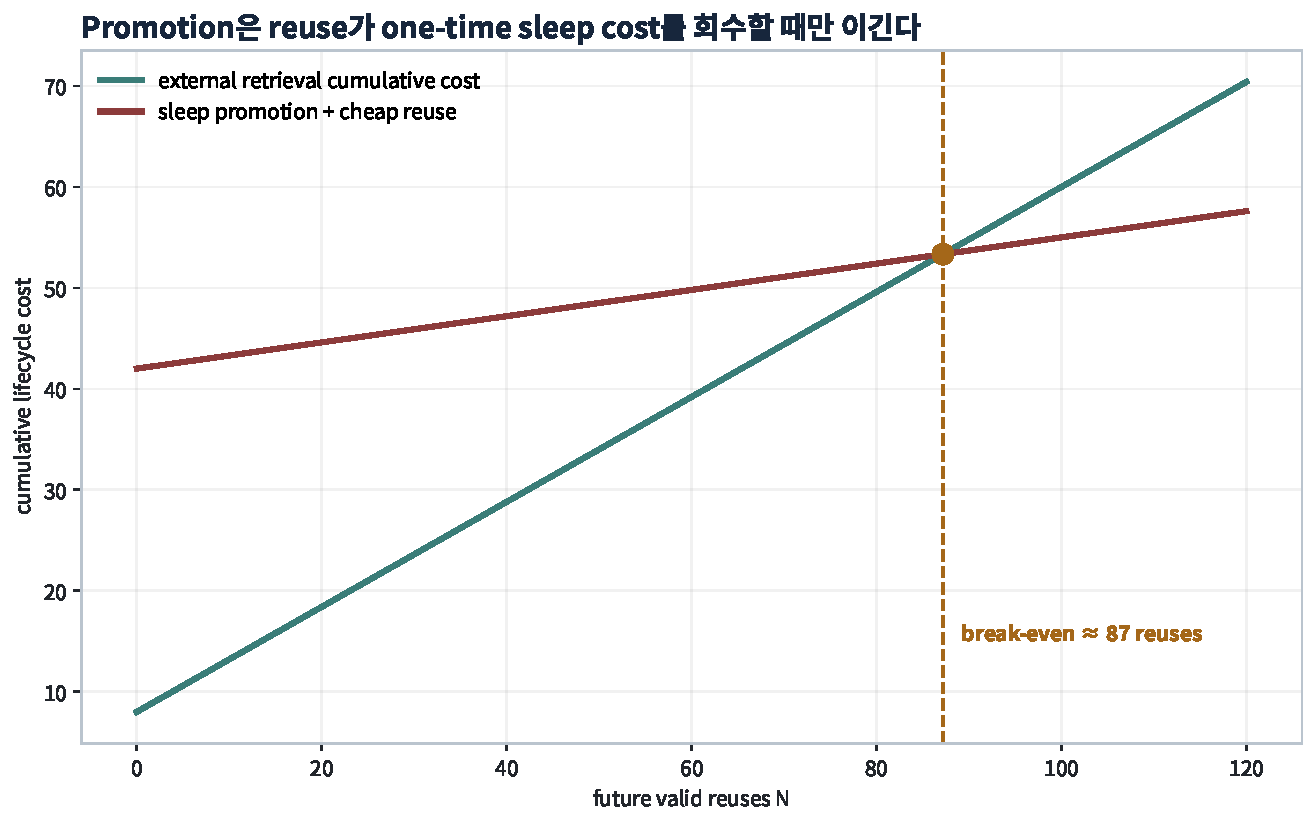
\includegraphics[width=0.96\textwidth]{figures/stc-f008.pdf}
  \caption{One-time sleep cost와 future valid reuse의 analytical crossover. Break-even 왼쪽은 external
  retrieval이, 오른쪽은 compiled artifact가 유리할 수 있다. Quality·governance 차이가 있으면 경계가
  이동한다.}
  \stcfigure{STC-F008}
  \figsource{Original analytical redraw; SRC-STC-0027, SRC-STC-0052}{초기 compile 비용을 수평선으로, reuse에 따라 누적되는 per-use saving을 상승선으로 나타낸 교차 그래프.}
  \label{fig:reuse-break-even}
\end{figure}

측정용 efficiency는 scalar를 강제하지 않고 먼저 Pareto vector로 보고한다.

\begin{align}
\eta_i={}&\frac{\Delta U_{later,i}\,R_{valid,i}}{C_{life,i}},\\
C_{life}={}&C_{ingest}+C_{transform}+C_{train}+C_{validate}\nonumber\\
&+C_{publish}+C_{serve}+C_{maint}+C_{delete/rollback}.
\end{align}

Dollar, joule, byte, second를 임의 환율로 합치지 않는다. Utility floor를 통과한 뒤 비용을 비교하거나,
cost cap 아래 utility를 비교하는 방식이 더 재현 가능하다.

\section{Finite state가 만드는 capacity knee}

고정된 finite state는 positive-entropy stream을 같은 distortion으로 영원히 보존할 수 없다. Mutable state가
$b_{mutable}$ bits이고 conditionally independent answer family의 rate--distortion cost가
$R_{Y_i\mid Q_i,\Theta_0}(D_i)$라면 제한된 조건 아래

\begin{equation}
\sum_{i=1}^{n}R_{Y_i\mid Q_i,\Theta_0}(D_i)
\le H(M_n\mid\Theta_0)\le b_{mutable}.
\end{equation}

이는 facts-per-parameter 보편 상수가 아니다. 하지만 계속 들어오는 novel evidence에 대해 state growth,
distortion 증가, forgetting, external offload 중 적어도 하나가 필요하다는 점은 분명히 한다.

Finite memory에서는 marginal consolidation utility가 떨어지고 interference, compaction 또는 delete cost가
급증하는 capacity knee가 나타날 것으로 예상된다.\claim{STC-C045}
\autocite{srcstc0034,srcstc0035,srcstc0036} Physical storage knee, normal-query reachability knee,
retrieval index knee, new-task plasticity knee, governance knee, hot-state residency knee는 서로 다른 위치에
있을 수 있다. 따라서 ``parameter가 아직 남았다''는 말은 behavioral capacity의 반증이 아니다.

\begin{figure}[htbp]
  \centering
  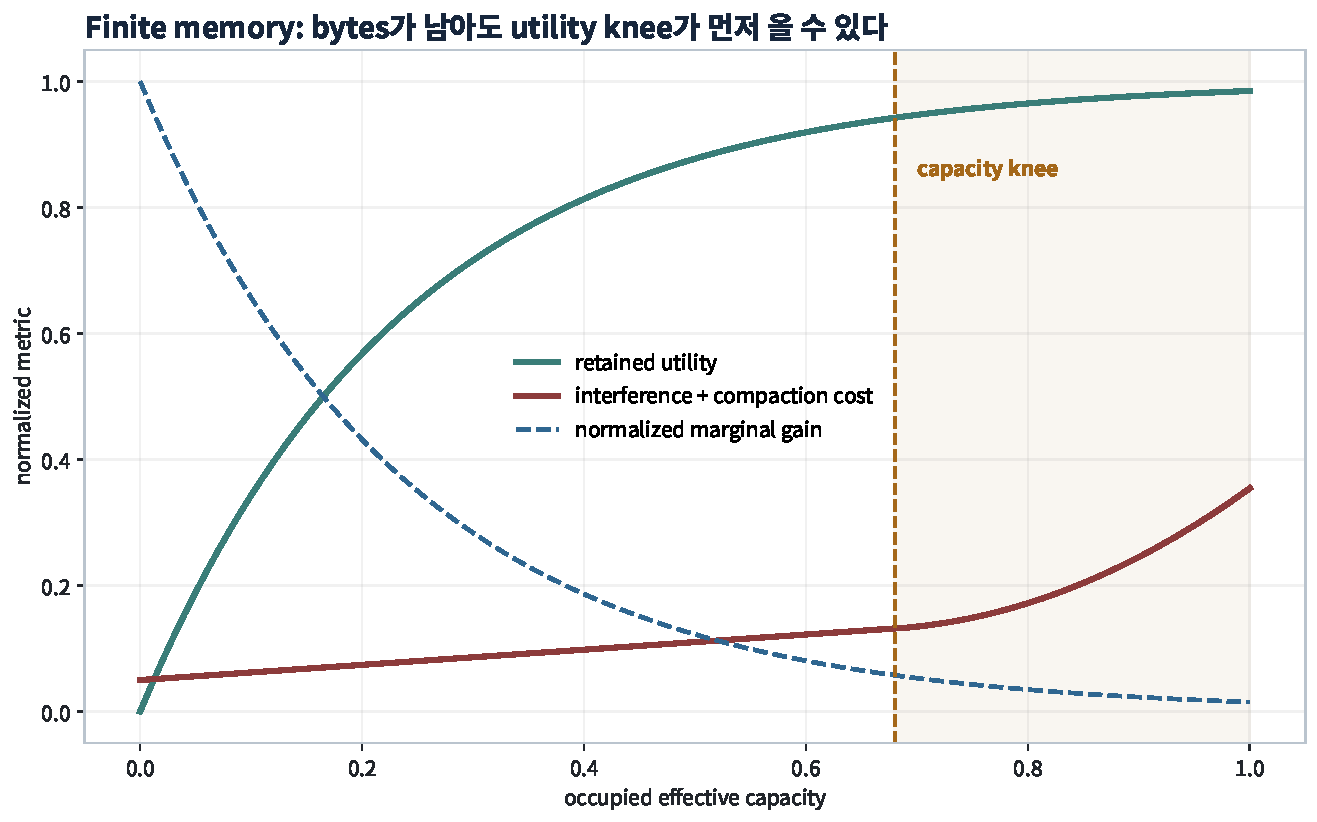
\includegraphics[width=0.96\textwidth]{figures/stc-f009.pdf}
  \caption{Finite-memory capacity knee의 가설적 형태. Physical occupancy가 한계에 닿기 전에 behavioral
  reachability 또는 plasticity가 임계값 아래로 내려갈 수 있다. 곡선은 설명용이며 측정 결과가 아니다.}
  \stcfigure{STC-F009}
  \figsource{Original hypothesis redraw; SRC-STC-0034, SRC-STC-0036}{Evidence load가 증가할 때 retention과 plasticity가 서로 다른 knee에서 감소하는 두 곡선.}
  \label{fig:capacity-knee}
\end{figure}

Controlled sweep에서는 retention threshold $\tau_{ret}$을 먼저 고정하고

\begin{equation}
\operatorname{logit}p_{ret}(N_a)=\operatorname{logit}\tau_{ret}
-\kappa\log(N_a/K_{eff})
\end{equation}

같은 segmented knee candidate와 generalized mean, min-bottleneck, monotone nonparametric competitor를
함께 맞춘다. 전 구간 power law 하나를 강제하지 않는다.

\section{Cadence와 queue의 내부 optimum}

Optimal cadence는 staleness, batching efficiency, interference와 wake-SLA impact를 균형시켜야 한다.
Continuous update나 무한히 긴 batch 어느 쪽도 일반적으로 최적이 아니다.\claim{STC-C044}
\autocite{srcstc0020,srcstc0022,srcstc0063}

Run cost $C_s$, interval $\tau$, smooth staleness penalty $a\tau^p$라는 제한에서

\begin{equation}
\bar C(\tau)=\frac{C_s}{\tau}+a\tau^p,
\qquad
\tau^*=\left(\frac{C_s}{ap}\right)^{1/(p+1)}.
\label{eq:cadence-optimum}
\end{equation}

Event rate $r_e$, fixed job cost $F$, linear delay harm $h$이면
$\tau^*=\sqrt{2F/(hr_e)}$다. Burst arrival, hard deadline, multi-resource blocking, capacity-triggered
regime change에서는 이 closed form이 깨진다. 이때 queue recursion
$Q_{t+1}=\max\{0,Q_t+A_t-S_t\}$와 P99 job age를 직접 시뮬레이션해야 한다.

\begin{figure}[htbp]
  \centering
  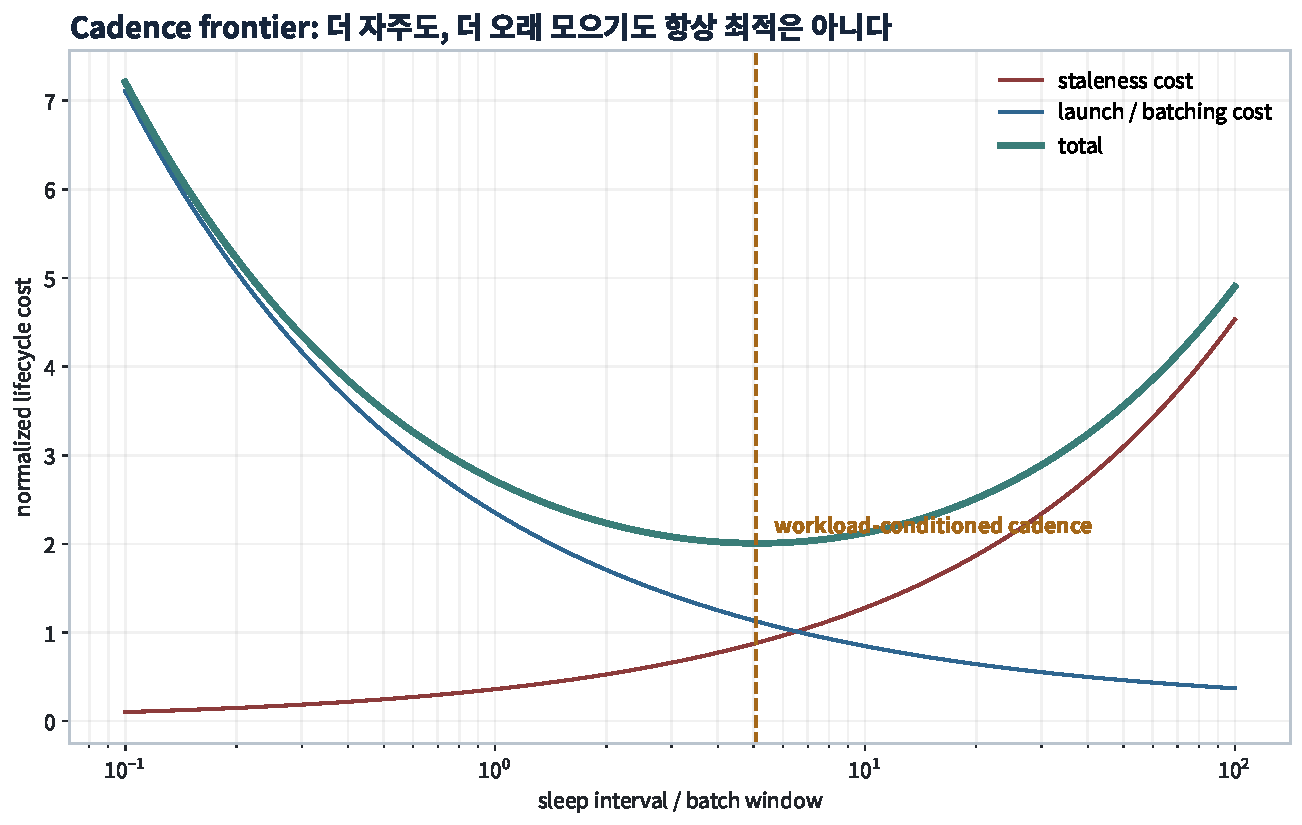
\includegraphics[width=0.96\textwidth]{figures/stc-f010.pdf}
  \caption{Cadence frontier. 너무 잦은 sleep은 fixed overhead와 interference가 크고, 너무 늦은 sleep은
  staleness와 queue age가 크다. 내부 optimum의 위치는 workload와 resource vector에 따라 변한다.}
  \stcfigure{STC-F010}
  \figsource{Original analytical redraw; SRC-STC-0020, SRC-STC-0063}{짧은 interval의 batching 비용과 긴 interval의 staleness 비용이 합쳐져 U자 total cost를 만드는 그래프.}
  \label{fig:cadence-frontier}
\end{figure}

\section{Fit candidate와 법칙 승격 조건}

첫 fit candidate는 saturating return에 interference, staleness, risk penalty를 분리한다.

\begin{equation}
\Delta U=A\left[1-\exp\left(-kF_s^{\alpha}E_{eff}^{\beta}R_v^{\gamma}\right)\right]
-\Phi_{int}-\Phi_{stale}-\Phi_{risk}.
\end{equation}

$E_{eff}$는 authorization, confidence, diversity를 통과한 canonical evidence이고 $R_v$는 valid future
reuse다. Competitor는 log-linear, floor가 있는 power law, segmented knee, generalized mean,
nonparametric monotone surface다. Sign change나 knee가 보이면 global power law를 기각한다.

진짜 STC scaling law라 부르려면 (1) unit과 state boundary를 고정하고, (2) model size·workload·medium·
hardware를 둘 이상 포함하며, (3) strongest alternative와 total lifecycle cost를 맞추고, (4) held-out
condition을 예측하고, (5) knee를 숨기지 않으며, (6) contamination·recursive depth·capacity·cycle control을
통과하고, (7) 실패한 형태를 공개해야 한다. 그 전까지의 정직한 산출물은 identity, restricted
break-even, workload-conditioned empirical surface와 falsifiable hypothesis다.
}{}
\IfFileExists{sections/13-infrastructure.tex}{\chapter{System infrastructure: wake, sleep, memory를 어떻게 잇는가}
\label{STC-S13}

세 개의 logical plane이 곧 세 개의 physical cluster를 뜻하지 않는다. 필요한 것은 latency-critical wake
execution, throughput-oriented candidate construction, transactional publication의 책임 분리다. Load와
state locality가 허용하면 같은 accelerator pool을 time-partition할 수 있고, contention 또는 privacy가
크면 분리할 수 있다. 배치는 brain analogy가 아니라 bytes, queue, SLO 측정으로 결정한다.

\section{세 plane과 하나의 publication transaction}

\begin{enumerate}
  \item \textbf{Wake plane}: inference, retrieval, optional fast learning, event append를 latency SLO 안에서
  수행하고, 하나의 authorized serving head를 pin한다.
  \item \textbf{Sleep plane}: immutable wake snapshot을 읽어 extract, compact, graph update, replay,
  distill, adapter tune, policy update, rebuild, verify job을 수행한다. 결과는 candidate일 뿐 live state가
  아니다.
  \item \textbf{Memory/control plane}: raw evidence와 derived views의 lineage, version, authorization,
  capacity, atomic publish, rollback을 관리한다.
\end{enumerate}

Sleep transaction은 다음처럼 표현할 수 있다.

\begin{equation}
T(X_v,M_v,B,P)\rightarrow \widehat M_{v+1}
\xrightarrow[\text{compare-and-swap}]{\text{validate}} M_{v+1}.
\label{eq:sleep-transaction}
\end{equation}

$X_v$는 immutable event range, $M_v$는 published manifest, $B$는 resource budget, $P$는 frozen policy다.
Candidate는 old/new/safety/delete/poison/system canary를 통과한 뒤에만 manifest-last로 publish된다.
Reader는 요청 중 한 version을 보며 partial vector/metadata/adapter state를 섞어 보지 않는다.

\section{Source-of-record와 heterogeneous materialized views}

Derived memory의 governance basis로는 updated weights 하나보다 external source-of-record와 provenance
graph가 강하다.\claim{STC-C046}\autocite{srcstc0053,srcstc0063,srcstc0066} Raw event도 retention
policy가 허용하는 동안만 canonical이다. Text summary, vector, graph, latent/KV, adapter, shared weight는
모두 source lineage를 가진 materialized view로 취급한다.

\begin{table}[htbp]
\centering
\caption{Memory medium별 serving path와 rollback contract}
\label{tab:medium-contract}
\begin{tabularx}{\textwidth}{L{0.18\textwidth} L{0.20\textwidth} Y L{0.24\textwidth}}
\toprule
Medium & Wake path & Update/validation & Rollback basis \\
\midrule
raw episode & selective retrieval & append, redact, expire & event/version log \\
semantic text & prompt injection & rewrite, faithfulness & source span + predecessor \\
vector/graph & ANN/traversal & re-embed, edge validity & index generation + episode \\
latent/recurrent & accelerator state read & compatibility, semantic probe & checkpoint or source rebuild \\
adapter/expert & model forward/router & train, merge, old/new canary & base digest + delta version \\
shared weight & model forward & full regression/unlearning & checkpoint + training lineage \\
\bottomrule
\end{tabularx}
\end{table}

삭제는 tombstone 한 번이 아니다. Immediate access deny, online artifact invalidation, derived lineage rebuild,
backup/key expiry, behavioral residual test를 서로 다른 deadline으로 기록한다. Old checkpoint 전체를 되살리는
rollback은 그 사이의 delete/consent epoch를 되돌릴 수 있으므로, authorized sub-root만 새 generation으로
재조합해야 한다.

\section{Scheduler: operator, destination, cadence를 분리한다}

하나의 evidence region에 대한 action space는 NO\_OP, RETAIN\_EXACT, EXPIRE, DEDUP, MERGE,
ABSTRACT, GRAPH\_UPDATE, LATENT\_COMPILE, ADAPTER\_COMPILE, PARAMETRIC\_PROMOTE, DEMOTE,
REBUILD, QUARANTINE를 포함한다. Learned policy가 action을 제안해도 privacy, tenant boundary,
capacity, deadline, promotion gate는 hard constraint로 남긴다.

Batching key는 base model/tokenizer와 adapter shape, embedding/index version, privacy zone, deadline,
operator, source shard다. 같은 batch가 효율적이라는 이유로 tenant security domain을 합치지 않는다.
Preemption은 uncommitted candidate를 버릴 수 있어야 하고, wake saturation 시 sleep보다 wake가 우선한다.

Sleep service는 scalar FLOP queue가 아니라 resource vector queue다.

\begin{equation}
\mathbf c_j=(c_{GPU\text{-}s},c_{CPU\text{-}s},c_{HBM\text{-}byte\text{-}s},
c_{RAM\text{-}byte\text{-}s},c_{IO\text{-}byte},c_{net\text{-}byte}).
\end{equation}

Mean GPU utilization이 낮아도 source affinity, validation model, index lock, network link 때문에 P99 job age가
발산할 수 있다. Queue 안정성은 utilization 한 숫자뿐 아니라 privacy deadline과 tenant starvation으로
판정한다.

\section{State migration roofline}

Separate sleep cluster는 training accelerator utilization을 높일 수 있지만 source episode, base model,
optimizer, adapter candidate, validation trace를 이동시킨다. Link $\ell$마다 이동 bytes $B_\ell$, transfer
price/energy $p_\ell$, delay $T_\ell$, delay value $v_{delay}$를 두면

\begin{equation}
C_{move}=\sum_{\ell}\left(B_\ell p_\ell+T_\ell v_{delay}\right).
\end{equation}

추가 local execution과 replication cost가 $C_{move}$보다 작을 때만 compute를 data 쪽으로 옮긴다.
Model/optimizer residency가 source보다 훨씬 크면 centralized GPU가, source-to-delta ratio와 privacy locality가
크면 shard-local preprocessing이 유리할 수 있다.

\begin{figure}[htbp]
  \centering
  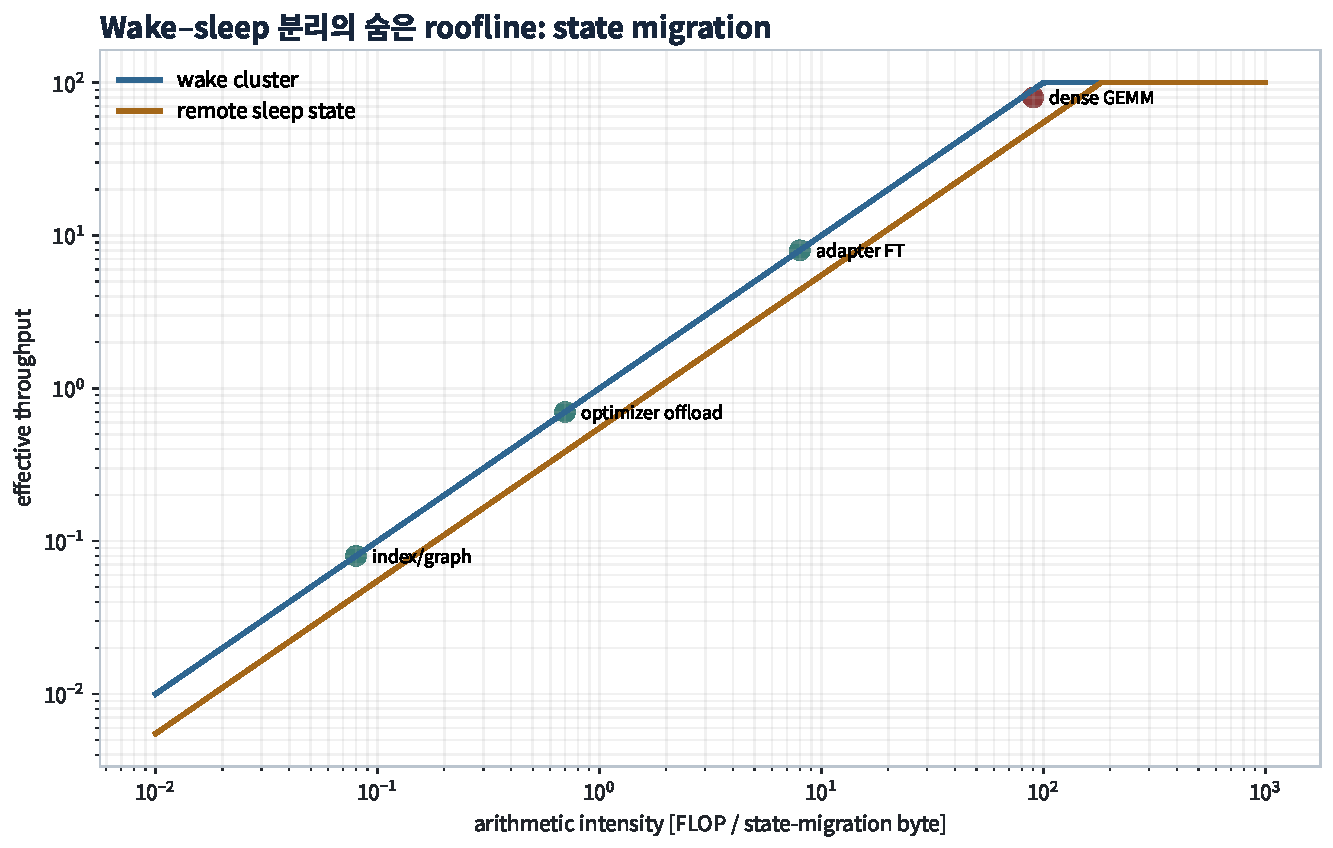
\includegraphics[width=0.97\textwidth]{figures/stc-f011.pdf}
  \caption{Wake/sleep placement의 state-migration roofline. Arithmetic intensity가 아니라 유용한 sleep
  work 대비 이동 state의 비율과 link bandwidth가 placement crossover를 정한다. 표시된 영역은 설계
  공간이며 특정 GPU의 측정 결과가 아니다.}
  \stcfigure{STC-F011}
  \figsource{Original systems synthesis; SRC-STC-0022, SRC-STC-0059}{Shared, separate, shard-local 배치를 state movement와 compute efficiency 축에서 비교한 roofline형 지도.}
  \label{fig:state-migration-roofline}
\end{figure}

\section{네 가지 physical placement}

\begin{longtable}{L{0.18\textwidth} L{0.22\textwidth} L{0.24\textwidth} L{0.21\textwidth}}
\caption{Physical placement option과 측정해야 할 trade-off}\label{tab:placement-options}\\
\toprule
Placement & 장점 & 비용/위험 & 적합 조건 \\
\midrule
\endfirsthead
\toprule
Placement & 장점 & 비용/위험 & 적합 조건 \\
\midrule
\endhead
shared priority fleet & base/model copy 최소, pooling & wake tail contention & sleep가 작고 preemptible \\
time-partitioned fleet & idle window 활용 & burst와 timezone mismatch & predictable diurnal load \\
separate wake/sleep & isolation, training batch 효율 & base replica와 network movement & sustained sleep demand \\
regional/shard-local hybrid & source locality, privacy & 낮은 local compute efficiency, fragmentation & source-to-delta ratio가 큼 \\
\bottomrule
\end{longtable}

\section{운영 계약}

Minimum viable system은 (1) append-only event log, (2) exact snapshot, (3) copy-on-write candidate,
(4) signed validation result, (5) atomic serving-head swap, (6) delete epoch와 deny root, (7) version-pinned
read, (8) bounded rollback과 GC owner를 가져야 한다. Algorithm quality가 좋아도 이 계약이 없으면 wake
request가 half-published state를 읽고, deleted source가 predecessor에서 부활하며, sleep retry가 duplicate
update를 만들 수 있다.

\begin{keypoint}[Infra 결론]
필요한 분리는 cluster의 개수가 아니라 responsibility와 transaction boundary다. Wake는 응답과 event
capture, sleep은 candidate construction, memory/control은 authoritative lineage와 publication을 담당한다.
Data 이동을 최소화한다는 말은 source만 보는 것이 아니라 base, optimizer, candidate, validation,
predecessor까지 같은 timestamp와 link에서 계측한다는 뜻이다.
\end{keypoint}
}{}
\IfFileExists{sections/14-device-opportunity.tex}{\chapter{Memory-device implication: 알고리즘 이름보다 workload primitive}
\label{STC-S14}

Memory-device 회사의 기회는 ``per-user weight sleep이 주류가 된다''는 한 시나리오에 종속되어서는 안
된다. External dominant, hybrid, periodic refresh, niche, broad adoption 모두에서 살아남는 traffic과
control primitive를 먼저 찾는다. 이 장은 market size나 제품 우위를 주장하지 않고, 측정해야 할
workload를 도출한다.

\begin{cautionbox}[Patent-first publication boundary]
Veridraft는 device 제품화에 관한 10개 P3 hypothesis를 internal/patent-first hold로 분류했다. 따라서
공개 claim ledger에는 해당 문장과 구현 세부를 싣지 않는다. 아래 내용은 이미 공개된 source에서 도출한
workload class와 evaluation question이며, 특정 제품 architecture나 권리 주장을 승인하는 문서가 아니다.
상세 opportunity matrix는 별도 내부 review를 거쳐야 한다.
\end{cautionbox}

\section{왜 inference memory와 다른 trace가 생기는가}

Fixed-model inference는 큰 weight의 read-mostly access, KV append/read, activation traffic이 중심이다.
Wake--sleep memory system은 여기에 네 종류를 추가한다.

\begin{enumerate}
  \item \textbf{Version traffic}: candidate, predecessor, snapshot, rollback reserve가 동시에 존재한다.
  \item \textbf{Index mutation}: vector payload, embedding key, graph edge, temporal validity가 함께 바뀐다.
  \item \textbf{Small-artifact fan-out}: user/cohort adapter, router catalog, recurrent state가 많아지고 hot set이
  시간에 따라 바뀐다.
  \item \textbf{Lineage control}: source handle, parent/replacement edge, delete epoch, validation attestation을
  low-tail-latency로 조회한다.
\end{enumerate}

따라서 peak bandwidth만 높인 장치보다 capacity, endurance, random metadata latency, copy-on-write,
atomic generation change, encryption domain, rebuild throughput의 조합이 중요해진다.

\begin{figure}[htbp]
  \centering
  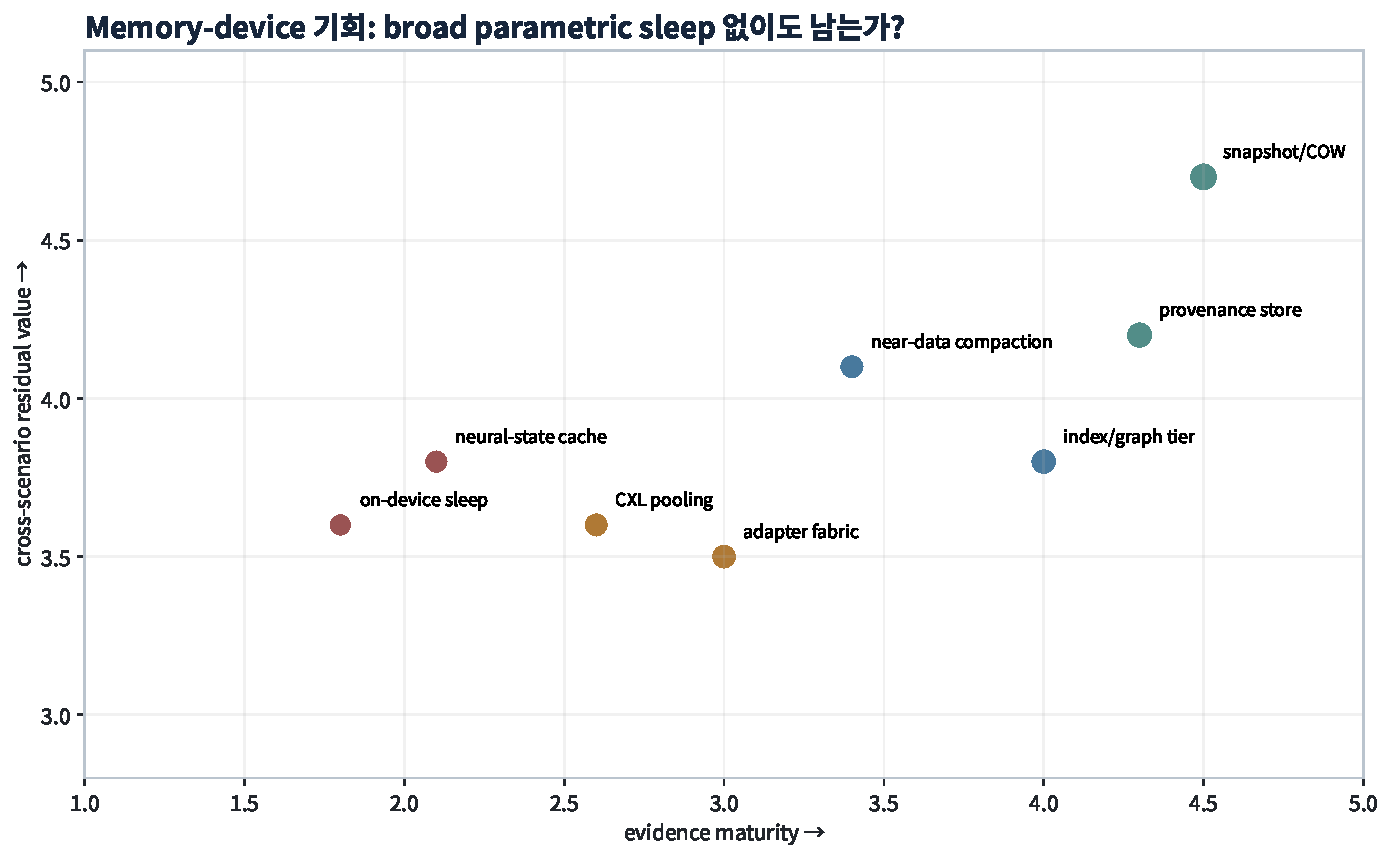
\includegraphics[width=0.97\textwidth]{figures/stc-f012.pdf}
  \caption{공개 source에서 관찰 가능한 workload class를 evidence maturity와 cross-scenario residual
  value의 두 축에 배치한 research map. 좌표는 제품 추천이나 시장 예측이 아니라 benchmark 우선순위를
  정하기 위한 정성적 가설이다.}
  \stcfigure{STC-F012}
  \figsource{Original research map; SRC-STC-0056, SRC-STC-0065}{Snapshot, provenance, mutable index, state cache, pooling, local compaction 등 workload 후보를 두 축에 놓은 산점도.}
  \label{fig:device-research-map}
\end{figure}

\section{Cross-scenario workload classes}

\begin{longtable}{L{0.18\textwidth} L{0.25\textwidth} L{0.22\textwidth} L{0.20\textwidth}}
\caption{Device 연구가 먼저 계측할 workload primitive}\label{tab:device-primitives}\\
\toprule
Class & Trace primitive & 시스템 가치 질문 & 비-STC residual value \\
\midrule
\endfirsthead
\toprule
Class & Trace primitive & 시스템 가치 질문 & 비-STC residual value \\
\midrule
\endhead
provenance episode & append, scan, sparse delete, lineage traversal & rebuild 범위와 audit latency를 줄이는가 & temporal RAG에도 높음 \\
snapshot/version & COW clone, multi-object publish, predecessor pin & rollback peak bytes/RTO를 줄이는가 & model/index release에도 높음 \\
mutable index/graph & small random rewrite, compaction, re-embed & write amplification과 tail latency는 얼마인가 & agent memory 전반에 높음 \\
state cache & recurrent/KV/adapter load, compatibility lookup & token prefix 외 state reuse를 회복하는가 & RNN/neural memory serving에 높음 \\
tiered pool & HBM--DRAM--CXL--storage migration & base duplicate와 state movement를 동시에 줄이는가 & inference와 refresh에도 높음 \\
local preprocessing & dedup, cluster, filter, graph maintenance & 이동 bytes/energy 절감이 local compute penalty보다 큰가 & data pipeline에도 중간--높음 \\
on-device idle work & burst train/compact, thermal pause, checkpoint & privacy benefit이 battery/endurance를 상쇄하는가 & local personalization에 높음 \\
lifecycle telemetry & per-item bytes, age, reuse, rollback, erase & useful retained evidence를 측정할 수 있는가 & 모든 memory system에 높음 \\
\bottomrule
\end{longtable}

\section{장치 요구사항을 metric으로 번역하기}

\textbf{Capacity.} Live state만이 아니라 candidate, pinned predecessor, migration duplicate, workspace,
replica를 포함한 $B_{peak,physical}(t)$를 측정한다. Snapshot 기능이 있어도 logical clone과 physical
dirty-page growth를 분리한다.

\textbf{Endurance.} Host write bytes뿐 아니라 device-level write amplification을 index/graph rewrite,
compaction, garbage collection, secure reclamation별로 분해한다. Update frequency가 서로 다른 CMS 또는
adapter tier는 한 평균 write rate로 합치지 않는다.

\textbf{Bandwidth와 locality.} Sequential episode scan, random ANN/graph access, checkpoint delta,
adapter page-in, validation readback을 각각 측정한다. Near-data operator는 saved link bytes와 추가 local
execution, model residency, result validation cost를 함께 보고한다.

\textbf{Tail latency.} Manifest, compatibility, lineage, deny-root lookup은 작은 I/O지만 wake request의
critical path에 있다. Bulk GB/s가 높아도 P99 metadata lookup이 길면 serving head를 안전하게 pin할 수
없다.

\textbf{Security와 recovery.} Tenant key boundary, instant deny, physical erase, stale replica discovery,
rollback-after-delete를 fault injection한다. Encryption throughput만으로 derived-state deletion을
증명하지 않는다.

\section{Device--system 공동 DSE}

하드웨어 design space exploration의 입력은 다음과 같이 workload에서 직접 온다.

\begin{equation}
\mathcal D=\{B_{source},B_{base},B_{delta},B_{index},B_{recovery},
R/W\ pattern,\tau_{cadence},Q_{age},R_v,\text{privacy locality}\}.
\end{equation}

출력은 later-wake utility floor 아래에서 total energy, bytes moved, write amplification, physical peak,
P99 wake interference, sleep completion age, rollback/delete time의 Pareto frontier다. 특정 장치가 sleep
job을 빨리 끝냈어도 base replica나 migration이 전체 비용을 키우면 system win이 아니다.

\section{의사결정 순서}

\begin{enumerate}
  \item 공개 trace와 simulator로 primitive를 먼저 검증한다.
  \item External-only와 periodic-refresh에도 가치가 남는 기능을 Tier 1으로 둔다.
  \item Hybrid/broad scenario에만 가치가 큰 state/adapter 기능은 leading indicator를 조건으로 둔다.
  \item Patentability, freedom-to-operate, security review가 끝나기 전에는 public claim으로 승격하지 않는다.
  \item 제품 KPI를 bandwidth가 아니라 useful retained evidence per lifecycle resource로 연결한다.
\end{enumerate}

\begin{keypoint}[Device 관점의 핵심]
가장 강건한 기회는 ``sleep training 전용 memory''라는 이름이 아니라, versioned derived state를 많이
만들고 검증하고 되돌리는 시스템의 memory primitive다. Parametric sleep이 지연되어도 provenance,
snapshot, temporal index, heterogeneous state caching과 lifecycle telemetry workload는 남는다.
\end{keypoint}
}{}
\IfFileExists{sections/15-benchmark-roadmap.tex}{\chapter{Falsifiable benchmark와 experiment roadmap}
\label{STC-S15}

이 분야에 필요한 다음 산출물은 더 큰 metaphor가 아니라 matched lifecycle experiment다. 같은 wake
events와 future queries를 주고, exact external retention, external compaction, latent/KV compilation,
user-local adapter, deliberate forgetting, past-only hybrid routing 중 무엇이 가장 나은지를 측정해야 한다.
Null result와 boundary를 계획에 포함해야 negative paper도 가치가 있다.

\begin{figure}[htbp]
  \centering
  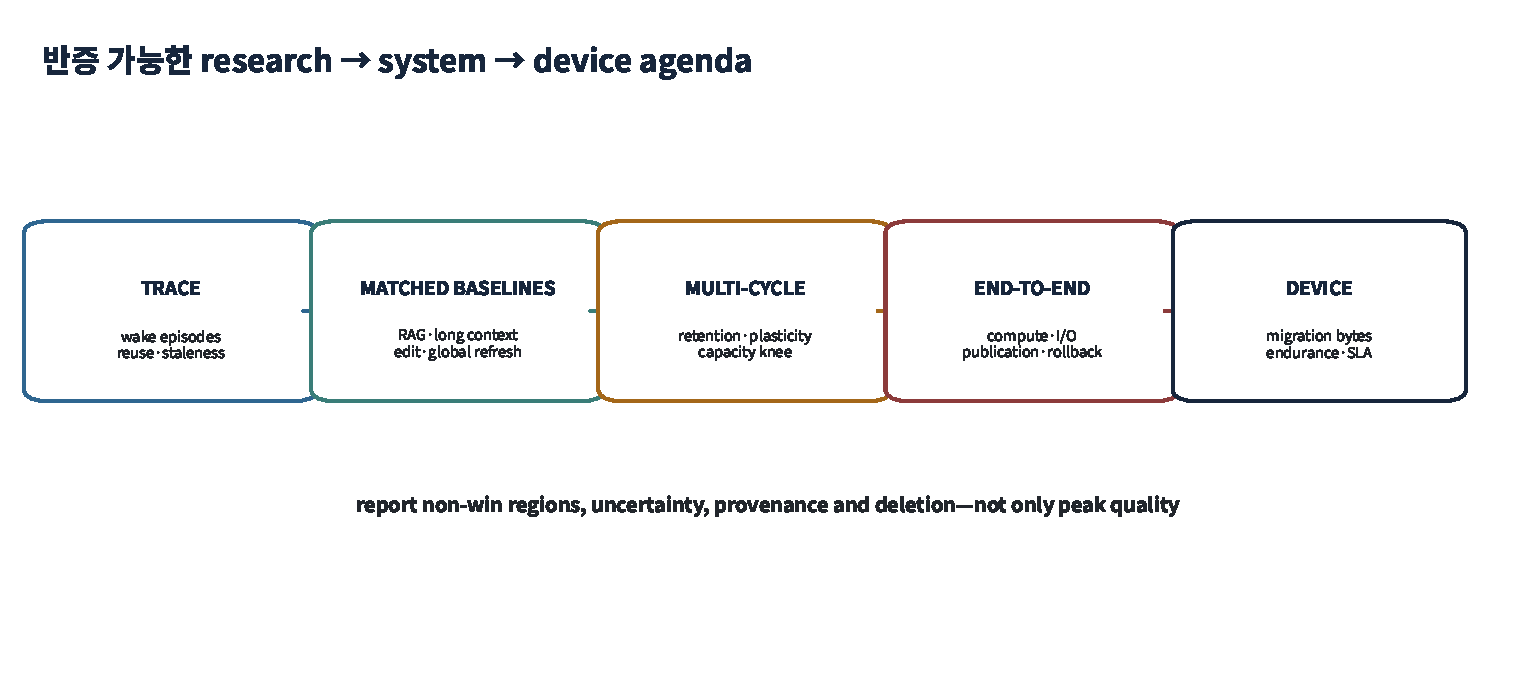
\includegraphics[width=0.98\textwidth]{figures/stc-f015.pdf}
  \caption{Falsifiable research agenda. Evidence stream, candidate construction, lifecycle validation,
  repeated-cycle evaluation, scaling fit을 하나의 provenance chain으로 연결한다.}
  \stcfigure{STC-F015}
  \figsource{Original synthesis; SRC-STC-0036, SRC-STC-0050, SRC-STC-0056}{Matched methods, cycle probes, systems/governance metrics, held-out scaling test가 순차적으로 이어지는 roadmap.}
  \label{fig:benchmark-agenda}
\end{figure}

\section{독립 단위와 cycle}

최상위 independent unit은 user/stream이다. Cycle과 probe를 독립 sample처럼 세어 significance를
부풀리지 않는다. 한 cycle은 다음 순서를 가진다.

\begin{align*}
\text{wake capture}&\rightarrow\text{pre-sleep probe}\rightarrow
\text{immutable snapshot}\rightarrow\text{candidate}\\
&\rightarrow\text{validate/publish}\rightarrow\text{post-sleep probe}
\rightarrow\text{delayed next-wake probe}.
\end{align*}

Default horizon은 128 cycles, sensitivity는 $C\in\{8,32,128,512\}$, retrieval lag는 가능한 경우
$\{1,8,32,128\}$ cycles로 둔다. 단일 sleep 후 정확도는 lifelong behavior를 지지하지 못한다.

\section{Observable과 oracle을 물리적으로 분리한다}

Method가 보는 observable stream에는 event payload, 현재 confidence, privacy scope, 알려진
supersession/delete, past reuse, resource/queue state만 있다. True future reuse, future contradiction,
future deletion, poison truth, ground-truth dependency, clairvoyant destination은 oracle ledger에 따로 둔다.
파일, schema, API permission과 process boundary로 누출을 막는다.

Train은 learned router/compiler를 fit하고, CALIBRATION은 threshold, cadence, baseline hyperparameter를
한 번 선택하며, TEST는 G2 freeze 뒤 한 번만 실행한다. TEST family identity나 future reuse로 configuration을
바꾸는 mutation test가 통과해야 한다. Dream-generated probe도 evaluation query가 아니라 derived training
artifact이므로 generator/prompt/input/output/filter digest를 남긴다.

\section{Event와 query family}

\begin{table}[htbp]
\centering
\caption{독립적으로 변화시킬 event factor와 주요 failure}
\label{tab:event-families}
\begin{tabularx}{\textwidth}{L{0.23\textwidth} L{0.34\textwidth} Y}
\toprule
Family & Controlled variables & 잡아야 할 failure \\
\midrule
stable exact fact & entropy, surface length, reuse, lag & semantic compression이 exact detail을 지움 \\
volatile fact/preference & validity interval, correction hazard & stale overwrite, historical loss \\
procedure/skill & reusable/one-off, environment version & vague summary, non-executable memory \\
relation/graph & alias, temporal edge, hop count & entity collision, invalid edge \\
failure feedback & wrong action, correction, avoidance & success-only bias \\
privacy/delete & consent expiry, dependency fan-out & tombstone-only delete \\
poison/adversarial & injection, conflicting frequency, delayed label & poison amplification \\
one-off distractor & salience, payload size, zero reuse & unnecessary consolidation \\
\bottomrule
\end{tabularx}
\end{table}

Reuse, volatility, poison, deletion, payload size와 memory pressure는 서로 독립적으로 변화시킨다. Query는
exact, semantic, temporal, relational, procedural, negative/failure, calibration, deletion family로 나눈다.
Acquisition query, exact repeat, held-out paraphrase, held-out composition, correction probe, unrelated control을
동일 지표로 합치지 않는다. ``기억한 문장을 그대로 다시 답했다''와 ``새 상황에 procedure를 적용했다''는
다른 능력이다.

\section{Confirmatory methods와 resource envelope}

Primary deployable family는 raw external, compressed external, latent/KV compiler, user-parametric LoRA,
static mixture, past-only hybrid router 여섯 개다. Clairvoyant oracle은 heterogeneity의 upper bound일 뿐
deployable method가 아니다. Long-context no-memory lower bound와 unbounded full-history upper bound는
diagnostic으로 남긴다.

모든 method는 다음 upper bound를 공유한다.

\begin{itemize}
  \item live token, active byte, durable byte, total incremental peak-state byte,
  \item physical HBM/fleet peak, sleep FLOPs, peak accelerator,
  \item 동일한 information cutoff, privacy와 delete contract.
\end{itemize}

Search/tuning, router, judge, embedding, synthetic data, optimizer, answer-reachable KV/recurrent state, index
rebuild, raw archive, lineage, rollback reserve와 transient workspace를 모두 charge한다. 사용하지 않은 budget은
낭비하도록 강제하지 않고 그대로 보고한다.

Reuse $R\in\{0,1,4,16\}$와 active-capacity ratio
$\phi\in\{1,1/4,1/16\}$을 교차한다. Schedule/operator factorial은 inline versus deferred와 identity
versus semantic consolidation을 destination external로 고정해, execution timing의 효과와 추가 정보를 더
본 효과를 분리한다.

\section{Metric stack}

\begin{longtable}{L{0.17\textwidth} L{0.74\textwidth}}
\caption{한 결과표에 함께 있어야 할 metric stack}\label{tab:benchmark-metrics}\\
\toprule
Layer & Required metrics \\
\midrule
\endfirsthead
\toprule
Layer & Required metrics \\
\midrule
\endhead
learning & lifetime utility AUC, current utility, acquisition, retention/forgetting, forward transfer, memory half-life \\
semantic & exact/semantic/temporal/relational/procedural, composition, relevance, calibration, false memory \\
memory path & writer/retriever/reader error, route/merge compatibility, coverage, faithfulness, detail loss, stale conflict \\
robustness & poison amplification, cross-user/task interference, rare-tail survival, recursive-depth distortion \\
governance & access deny, physical removal, lineage invalidation, key expiry, behavioral residual, rollback success/time \\
serving & TTFT/ITL/task P50/P95/P99, throughput, cache/adapter hit, load/swap, fallback \\
sleep service & throughput, queue age, deadline miss, retry, validation/publish/rollback cost \\
resources & pre/post/wake/sleep/validation FLOPs, retained/peak bytes, bytes moved by link, write amplification, energy \\
compatibility & base/tokenizer/embedding version, artifact route, rebase and rebuild cost \\
\bottomrule
\end{longtable}

Primary quality endpoint은 cycle과 pre/post/delayed probe block에 동일 가중치를 주는 lifetime utility AUC다.
Energy-per-correct는 frozen accuracy floor 위에서만 계산한다. Delete score는 access denial과 physical removal,
derived invalidation, behavioral residual을 한 binary로 합치지 않는다.

\section{통계·재현성과 claim-down rule}

모든 method는 같은 stream, event order, query order, resource tuple을 받는다. User/stream을 paired resampling
unit로 사용하고 workload-family$\times$seed-family block을 유지한다. Hardware placement와 method order는
randomize 또는 block한다. Outcome을 본 뒤 stopping point, comparator, hypothesis family를 바꾸지 않는다.

Run artifact는 source/version $\rightarrow$ question/hypothesis $\rightarrow$ config/data/code/environment
$\rightarrow$ raw checksum $\rightarrow$ result $\rightarrow$ claim $\rightarrow$ figure/table
$\rightarrow$ manuscript sentence를 연결한다. Timeout, OOM, deadline miss, cap violation은 missing data가
아니라 consumed work를 charge한 RESOURCE\_FAILURE로 처리한다.

다음 경우 claim을 낮춘다: effect가 materiality margin보다 작음, equivalence interval이 margin을 걸침,
simulation으로 absolute hardware latency를 말함, archive를 남기고 total compression이라 함, behavioral
forgetting을 physical deletion이라 함, post-hoc arm을 추가함. Minimum publishable result는 hybrid가
실패해도 deterministic leakage-tested stream, matched methods, complete resource ledger, retention/acquisition
분리와 잘 추정된 crossover·knee·null 중 하나를 남기는 것이다.

\begin{keypoint}[실험의 최종 질문]
``Sleep이 정확도를 높였는가?''가 아니라 ``동일한 evidence와 lifetime budget에서, 어떤 admission,
operator, destination, cadence가 later-wake utility와 governance의 Pareto frontier를 움직였는가?''를 묻는다.
\end{keypoint}
}{}
\IfFileExists{sections/16-limitations-falsifiers.tex}{\chapter{Limitations, negative evidence와 falsifiers}
\label{STC-S16}

이 Study의 결론은 2026-08-05 공개 evidence에 대한 조건부 synthesis다. Product 내부 trace, 비공개
deployment incident, 실제 device workload가 없으며, 논문 간 model·task·budget이 달라 meta-analysis를
수행하지 않았다. Original figure의 좌표와 scenario는 측정 결과가 아니라 reasoning aid다.

\section{문헌 자체의 한계}

명시적 parametric sleep 연구는 direct mechanism evidence지만 model scale, task diversity, cycle count와
production governance가 제한된다. Product documentation은 background phase의 존재를 보여도 strongest
alternative 대비 causal advantage를 보여 주지 않는다. Continual-learning precursor는 forgetting을 줄이는
방법을 제공하지만 LLM agent의 deletion, state migration, future reuse economics를 직접 측정하지 않는다.

DANN/SSRN record는 동결 source에서 independent verification에 필요한 method와 result를 충분히 공개하지
않아 load-bearing evidence로 사용하지 않았다.\claim{STC-C047}\autocite{srcstc0039} 제목이나 abstract가
``zero forgetting''을 말해도 full method, data, comparator, statistics, artifact가 없으면 central claim을
지탱할 수 없다. 이 판단은 논문이 틀렸다는 결론이 아니라 증거 접근성에 대한 claim-down이다.

\section{Negative evidence가 가리키는 구조적 위험}

\begin{longtable}{L{0.20\textwidth} L{0.31\textwidth} L{0.39\textwidth}}
\caption{실패 mode와 필요한 control}\label{tab:negative-evidence}\\
\toprule
Risk & 관찰/이론적 근거 & 필요한 control \\
\midrule
\endfirsthead
\toprule
Risk & 관찰/이론적 근거 & 필요한 control \\
\midrule
\endhead
behavioral unreachability & sequential fact가 weights에 남아도 normal query에서 접근 불가 & direct, prompted, compositional reachability를 분리 \\
catastrophic interference & new update가 old task와 plasticity를 손상 & old/new/safety slice, replay/regularization/isolation ablation \\
recursive-data collapse & synthetic-only generations가 rare tail을 잃을 수 있음 & canonical anchor, recursive depth, common/tail distortion \\
false merge/compaction & summary가 exact, temporal, negative detail을 지움 & source spans, faithfulness, exact/temporal query, rebuild \\
memory poisoning & persistent record가 후속 behavior를 조종 & provenance, quarantine, poison canary, least privilege \\
delete illusion & tombstone 뒤 summary, index, cache, adapter에 영향 잔존 & lineage fan-out, deny root, physical removal, residual probe \\
state fan-out & user/cohort artifact와 catalog가 base saving을 상쇄 & total state, hot residency, route/load latency \\
queue/SLA failure & 평균 utilization 전에도 affinity·validation이 P99 age를 악화 & multi-resource queue, deadline, wake preemption \\
version churn & base/tokenizer/embedding 변경이 artifact를 무효화 & compatibility digest, rebase/rebuild cost \\
\bottomrule
\end{longtable}

\begin{figure}[htbp]
  \centering
  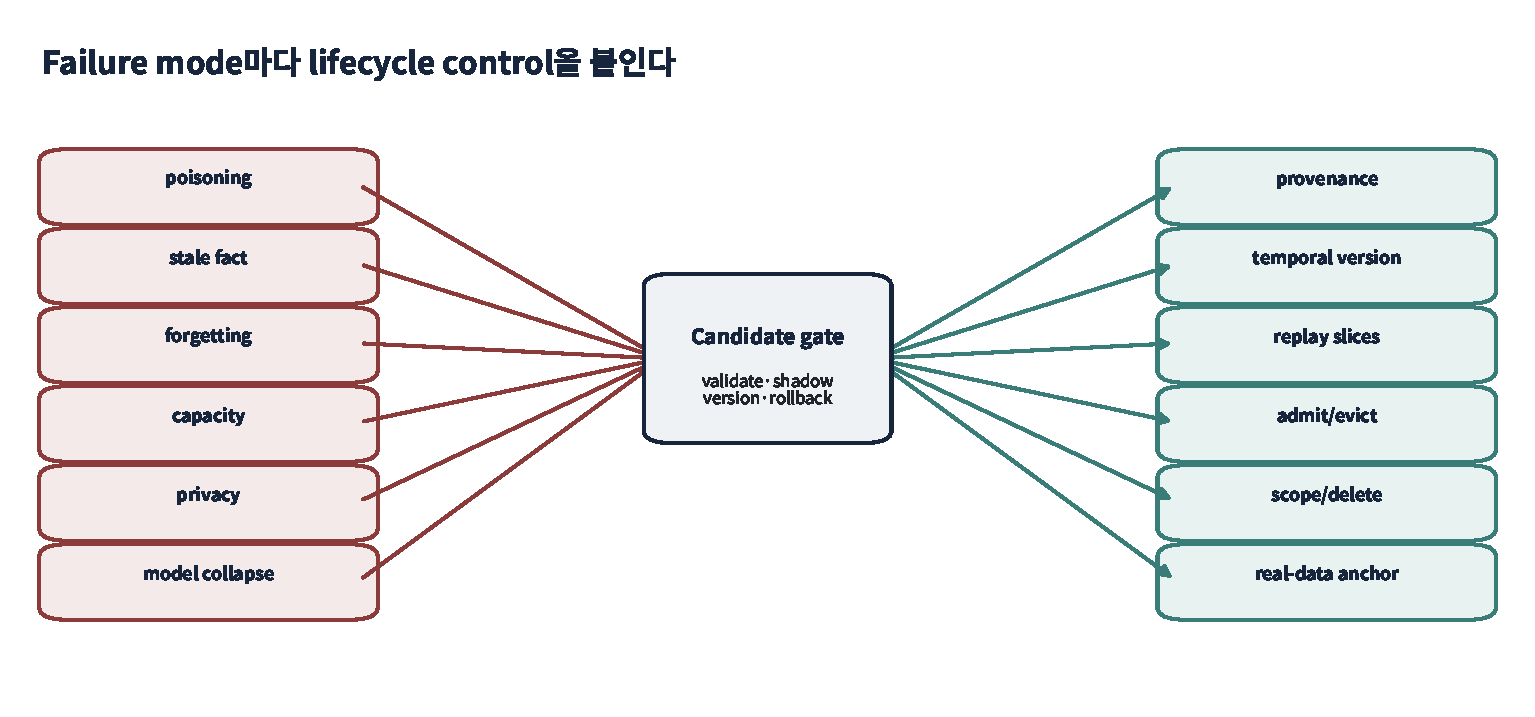
\includegraphics[width=0.98\textwidth]{figures/stc-f013.pdf}
  \caption{Wake capture에서 deletion까지 이어지는 주요 failure mode와 lifecycle control. 한 단계의
  accuracy gate만으로는 poison, stale publish, rollback resurrection, residual delete를 막을 수 없다.}
  \stcfigure{STC-F013}
  \figsource{Original synthesis; SRC-STC-0042, SRC-STC-0053}{Admission, candidate, publish, serve, delete 단계마다 poison·interference·race·residual과 대응 control을 연결한 흐름도.}
  \label{fig:failure-controls}
\end{figure}

\section{결론을 뒤집거나 좁힐 구체적 falsifier}

\textbf{F1---새 phase claim.} 동일 transformation, information cutoff, destination, total resource를
맞췄을 때 deferred와 synchronous 실행의 later-wake quality, wake-SLA, batching 차이가 모두 사라지면
``새 scientific axis''는 scheduling label로 좁혀야 한다.

\textbf{F2---hybrid recommendation.} External-only 또는 direct parametric-only가 stable skill과 volatile
fact 모두에서 utility, cost, deletion, rollback, portability를 지배하면 hybrid default를 폐기한다.

\textbf{F3---valid-reuse hypothesis.} Reuse와 query predictability를 넓게 sweep해도 STC gain과 interaction이
없거나 predictor error가 top-$k$ yield를 없애면 reuse-based promotion 이론을 기각한다.

\textbf{F4---capacity knee.} Repeated stream에서 behavioral retention/plasticity가 physical occupancy와
같이 부드럽게 변하고 앞선 knee가 재현되지 않으면 별도 behavioral knee hypothesis를 기각한다.

\textbf{F5---canonical anchoring.} Synthetic/summary replay와 source-anchored replay의 rare-tail survival이
matched cost에서 차이가 없으면 canonical anchor의 안정성 주장을 낮춘다.

\textbf{F6---dedicated sleep infra.} Shared priority fleet가 모든 realistic trace에서 더 낮은 physical
peak, 이동 bytes, P99 wake latency와 job age를 동시에 보이면 separate sleep cluster 필요성을 기각한다.

\textbf{F7---device relevance.} Background memory job이 commodity CPU/object-store metadata 수준에 머물고
retained bytes, rewrite, movement, tail-SLA가 장치 선택에 영향을 주지 않으면 새로운 memory workload라는
주장을 좁힌다.

\section{Coverage와 saturation의 한계}

Search cluster는 date-bounded snapshot이며 five active frontier와 five measurement gap을 명시적으로
남겼다. 특히 Google, Meta, Microsoft의 research output은 넓지만 public production per-user weight sleep의
부재를 ``그 회사가 하지 않는다''는 negative fact로 바꾸지 않는다. 공개하지 않았을 가능성과 아직
측정하지 않은 possibility가 있기 때문이다.

Figure는 권리 검토된 original redraw만 사용했으며 source paper figure를 직접 복제하지 않았다. 이
선택은 copyright risk를 줄이지만 원 실험 plot의 numeric fidelity를 대신하지 않는다. 독자는 claim
ledger와 primary source로 수치를 확인해야 한다.

\section{본 논문이 주장하지 않는 것}

\begin{itemize}
  \item Biological NREM/REM stage가 AI operator에 one-to-one으로 대응한다는 주장,
  \item 더 많은 sleep FLOPs가 항상 utility를 높인다는 universal monotone law,
  \item weights가 external memory보다 본질적으로 더 장기적이라는 주장,
  \item 공개 product lifecycle가 comparative scientific optimality를 입증한다는 주장,
  \item simulation이 특정 GPU·memory device의 latency, energy, endurance를 측정했다는 주장,
  \item P3-held device hypothesis가 publication 또는 patent review를 통과했다는 주장.
\end{itemize}

\begin{cautionbox}[가장 중요한 한계]
현재 논문은 measurement program과 conditional strategy를 제시한다. STC의 universal dominance나 broad
parametric deployment를 관측한 논문이 아니다. 이 구분을 유지해야 향후 negative result가 연구 실패가
아니라 이론의 경계를 좁히는 결과가 된다.
\end{cautionbox}
}{}
\IfFileExists{sections/17-conclusion.tex}{\chapter{Conclusion: 다음 학습 축의 조건과 연구 순서}
\label{STC-S17}

본 연구의 답은 단순한 찬반이 아니다. Sleep-time compute은 release-time pre/post-training과
latency-critical test-time learning 사이에, accumulated wake experience를 reusable later-wake state로
바꾸는 deferred lifecycle budget을 추가한다. 이 기능적 축은 이미 external background synthesis에서
product evidence를 갖는다. 그러나 broad per-user foundation-weight sleep이 주류가 되거나 보편 scaling
law를 가진다는 증거는 없다.

\section{처음의 질문에 대한 직접 답}

\textbf{무슨 문제를 푸는가?} Static deployment와 persistent agent experience 사이의 간극, 반복되는 long
context 비용, cross-session strategy learning, freshness/contradiction, finite-memory compaction, wake latency와
learning throughput의 충돌을 푼다. 하나의 method가 이 문제를 모두 풀지는 않는다.

\textbf{Sleep이 최선인가?} One-off document, exact volatile fact, unpredictable query에는 long context,
RAG와 temporal external memory가 더 강하다. Stable high-reuse procedure, multi-episode pattern,
background conflict resolution에서는 deferred transformation이 유망하다. Continual learning에서는 sleep이
replay, regularization, isolation, validation을 실행하는 phase를 제공할 뿐 capacity theorem을 없애지 않는다.

\textbf{Parametric인가 external인가?} Binary choice가 아니다. External source-of-record에 canonical
evidence와 provenance를 보존하고, calibrated reuse와 stability가 충분한 subset만 reversible parametric
artifact로 compile하는 hybrid가 현재 가장 방어적이다. Changing fact, deletion-sensitive episode,
low-reuse item은 external에 남는다.

\textbf{업계와 학계는 어디로 가는가?} 업계는 external synthesis, provenance, control과 background job으로,
학계는 learned memory writer/router, neural fast state, continual-learning mechanism, compaction theory와
benchmarks로 수렴한다. Lifecycle이 mainstream이 되어도 이름은 dreaming, reflection, synthesis 또는
memory로 남을 수 있다.

\textbf{Scaling law는 무엇인가?} 지금은 법칙이 없다. 먼저 complete state/work identity, reuse와 cadence의
restricted break-even, capacity knee와 state-migration crossover를 측정한다. 그다음 evidence quality,
valid reuse, cycle count, recursive depth, medium, hardware를 교차한 held-out predictive surface가 반복되면
비로소 제한된 scaling law를 말할 수 있다.

\textbf{Memory-device 회사의 기회는 무엇인가?} 특정 parametric sleep adoption에 베팅하기보다 versioned
derived state, provenance, temporal index, snapshot/rollback, heterogeneous state cache, state-local processing,
lifecycle telemetry의 실제 trace를 공동 측정해야 한다. 상세 제품 hypothesis는 patent-first review 뒤에
공개한다.

\section{권장 연구 순서}

\begin{enumerate}
  \item \textbf{External lifecycle baseline}: versioned raw/summary/vector/graph와 exact delete/rollback을 먼저
  구현해 source-of-truth와 metric을 고정한다.
  \item \textbf{Matched benchmark}: 동일 event/query/resource에서 raw, compressed, latent, LoRA, static
  mixture, past-only router를 128+ cycles 비교한다.
  \item \textbf{Reuse/capacity sweep}: $R$, volatility, active capacity, recursive depth, cadence를 독립적으로
  변화시켜 crossover와 knee를 찾는다.
  \item \textbf{Selective promotion}: stable procedural subset에만 versioned adapter/latent compile을 허용하고
  rebase, demotion, delete fault를 주입한다.
  \item \textbf{Trace-driven infra DSE}: shared, time-partitioned, separate, shard-local placement에서 base
  residency와 모든 state-migration bytes를 계측한다.
  \item \textbf{Device co-design}: public trace로 capacity, endurance, tail latency, COW, secure reclamation의
  sensitivity를 검증한 뒤 product research로 승격한다.
\end{enumerate}

\section{마지막 framing}

앞으로의 학습을 세 phase로 보는 framing은 유용하다.

\begin{align*}
\underbrace{\text{pre/post-training}}_{\text{release 전 shared capability}}
&\rightarrow
\underbrace{\text{test-time learning}}_{\text{wake adaptation}}\\
&\rightarrow
\underbrace{\text{sleep-time learning}}_{\text{deferred consolidation}}
\rightarrow
\underbrace{\text{versioned long-term memory}}_{\text{later-wake reuse}}.
\end{align*}

다만 화살표는 일방향이 아니다. Delete와 correction은 long-term memory에서 derived state로 역전파되고,
base release는 adapter와 index를 재검증하며, wake failure는 다음 sleep candidate를 만든다. 미래의 scaling
object는 checkpoint 하나가 아니라 여러 clock과 memory medium, provenance와 transaction을 가진 system일
가능성이 높다.

\begin{keypoint}[최종 verdict]
Sleep-time compute은 promising한 새 lifecycle 축이지만, 현재의 승자는 broad weight update가 아니라
external background consolidation이다. 가장 유망한 다음 단계는 external source-of-record 위의 selective,
reversible promotion이며, 그 가치는 sleep FLOPs가 아니라 valid later-wake reuse per complete lifecycle
resource로 검증해야 한다.
\end{keypoint}
}{}

\appendix
\IfFileExists{tables/claim-table.tex}{% Generated from claims/stc-study/claim-map.json. Do not edit by hand.
\chapter*{Canonical claim–evidence ledger}
\addcontentsline{toc}{chapter}{Canonical claim–evidence ledger}
\markboth{Canonical claim–evidence ledger}{Canonical claim–evidence ledger}
본문의 파란 claim ID는 이 표의 canonical English statement와 source locator로 연결된다.
이 표는 번역문이 아니라 Veridraft gate를 통과한 frozen assertion surface다.

\scriptsize
\begingroup
\setlength{\tabcolsep}{3pt}
\begin{longtable}{p{0.105\textwidth} p{0.105\textwidth} p{0.455\textwidth} p{0.245\textwidth}}
\caption{Veridraft-gated public claims (source freeze 2026-08-05)}\label{tab:claim-ledger}\\
\toprule
ID & Type / confidence & Canonical claim & Evidence locator \\
\midrule
\endfirsthead
\toprule
ID & Type / confidence & Canonical claim & Evidence locator \\
\midrule
\endhead
\midrule\multicolumn{4}{r}{다음 쪽에 계속}\\
\endfoot
\bottomrule
\endlastfoot
\hypertarget{claim-ledger:STC-C001}{\hyperlink{claim:STC-C001}{\textbf{STC-C001}}} & direct fact\newline high & The date-frozen evidence audit contains 73 primary papers, official releases, documentation pages, and tagged repositories. & \texttt{SRC-STC-0014}: source registry audit; entry SRC-STC-0014 \\
\hypertarget{claim-ledger:STC-C002}{\hyperlink{claim:STC-C002}{\textbf{STC-C002}}} & direct fact\newline high & By 2026-08-05, at least two public production systems described explicit background memory synthesis: OpenAI Dreaming and Mem0 Dream. & \texttt{SRC-STC-0052}: official release, opening and How dreaming works\newline \texttt{SRC-STC-0063}: official docs, Overview and How Dream works \\
\hypertarget{claim-ledger:STC-C003}{\hyperlink{claim:STC-C003}{\textbf{STC-C003}}} & direct fact\newline high & The 12-cluster search closes only as a bounded date snapshot: 2 clusters are bounded, 5 remain active frontiers, and 5 retain measurement gaps. & \texttt{SRC-STC-0036}: paper abstract and §5 limitations \\
\hypertarget{claim-ledger:STC-C004}{\hyperlink{claim:STC-C004}{\textbf{STC-C004}}} & direct fact\newline high & A balanced 15-paper translation corpus spans explicit sleep, biological and computational precursors, continual learning, external memory, neural memory, capacity, and negative evidence. & \texttt{SRC-STC-0011}: full paper, title through Discussion \\
\hypertarget{claim-ledger:STC-C005}{\hyperlink{claim:STC-C005}{\textbf{STC-C005}}} & synthesis\newline high & Sleep-time compute is best defined by lifecycle, not by metaphor: computation is deferred beyond the latency-critical response and changes reusable state for later wake episodes. & \texttt{SRC-STC-0014}: abstract; §1; Fig. 1\newline \texttt{SRC-STC-0052}: official release, How dreaming works\newline \texttt{SRC-STC-0063}: official docs, Synthesis mode \\
\hypertarget{claim-ledger:STC-C006}{\hyperlink{claim:STC-C006}{\textbf{STC-C006}}} & synthesis\newline high & Update timing and memory medium are orthogonal axes: a sleep phase may update weights, adapters, recurrent state, text/vector stores, graphs, or mixtures. & \texttt{SRC-STC-0014}: §2, sleep-time agent architecture\newline \texttt{SRC-STC-0021}: §2-§3, self-modification and consolidation\newline \texttt{SRC-STC-0016}: §2-§3, temporal graph memory \\
\hypertarget{claim-ledger:STC-C007}{\hyperlink{claim:STC-C007}{\textbf{STC-C007}}} & direct fact\newline high & OpenAI Dreaming is production background synthesis over external user memory, not disclosed per-user foundation-weight training. & \texttt{SRC-STC-0052}: official release, opening through How dreaming works \\
\hypertarget{claim-ledger:STC-C008}{\hyperlink{claim:STC-C008}{\textbf{STC-C008}}} & direct fact\newline high & Mem0 Dream performs scheduled background synthesis with provenance-preserving, additive outputs; merge and supersede are distinct ingest-time operations. & \texttt{SRC-STC-0063}: official docs, Overview; Modes; Operational behavior\newline \texttt{SRC-STC-0064}: tag v2.0.13, dream-gate.ts \\
\hypertarget{claim-ledger:STC-C009}{\hyperlink{claim:STC-C009}{\textbf{STC-C009}}} & direct fact\newline high & Letta's tagged sleeptime group schedules an asynchronous post-response agent that revises durable memory outside the response-critical path. & \texttt{SRC-STC-0059}: tag 0.16.8, sleeptime\_multi\_agent\_v4.py \\
\hypertarget{claim-ledger:STC-C010}{\hyperlink{claim:STC-C010}{\textbf{STC-C010}}} & direct fact\newline high & Zep and Graphiti represent external memory as temporally versioned episodes, entities, and relations rather than as user-specific model-weight updates. & \texttt{SRC-STC-0016}: abstract; §2 Architecture; §3 Temporal KG\newline \texttt{SRC-STC-0065}: commit aab852d, README overview\newline \texttt{SRC-STC-0066}: official docs, Episodes \\
\hypertarget{claim-ledger:STC-C011}{\hyperlink{claim:STC-C011}{\textbf{STC-C011}}} & author claim\newline high & MemGPT frames long-term agent memory as an operating-system-style hierarchy that pages information between constrained context and external storage. & \texttt{SRC-STC-0013}: abstract; §2 Virtual Context Management; Fig. 1 \\
\hypertarget{claim-ledger:STC-C012}{\hyperlink{claim:STC-C012}{\textbf{STC-C012}}} & direct fact\newline high & ReasoningBank stores reusable reasoning strategies extracted from experience; the public method is an external strategy memory rather than broad online weight consolidation. & \texttt{SRC-STC-0043}: abstract; §2-§3\newline \texttt{SRC-STC-0054}: official Google Research post, Method \\
\hypertarget{claim-ledger:STC-C013}{\hyperlink{claim:STC-C013}{\textbf{STC-C013}}} & synthesis\newline medium & Meta's personalized-agent and HyperAgents work emphasizes feedback-conditioned agent behavior, program memory, and archives; public evidence does not establish fleet-scale per-user sleep updates to foundation weights. & \texttt{SRC-STC-0057}: official Meta paper page, abstract\newline \texttt{SRC-STC-0058}: official Meta paper page, abstract \\
\hypertarget{claim-ledger:STC-C014}{\hyperlink{claim:STC-C014}{\textbf{STC-C014}}} & direct fact\newline high & Microsoft STATE-Bench evaluates agent memory across state tracking, adaptation, and efficiency, but is a benchmark rather than a disclosed sleep-training product. & \texttt{SRC-STC-0056}: official Microsoft post, benchmark dimensions\newline \texttt{SRC-STC-0067}: commit 4efcbf2, README tasks and metrics \\
\hypertarget{claim-ledger:STC-C015}{\hyperlink{claim:STC-C015}{\textbf{STC-C015}}} & synthesis\newline high & Language Models Need Sleep is direct evidence for parametric sleep: the model learns to self-modify and consolidate memories using replay-like training, but the reported regime remains research-scale rather than production deployment proof. & \texttt{SRC-STC-0021}: abstract; §2 Method; §4 Experiments; §6 Limitations \\
\hypertarget{claim-ledger:STC-C016}{\hyperlink{claim:STC-C016}{\textbf{STC-C016}}} & author claim\newline high & In a two-task spiking-network setting, interleaved sleep-like replay formed a joint synaptic representation and reduced catastrophic forgetting. & \texttt{SRC-STC-0011}: abstract; Results, Figs. 2-7; Discussion \\
\hypertarget{claim-ledger:STC-C017}{\hyperlink{claim:STC-C017}{\textbf{STC-C017}}} & author claim\newline high & A hippocampus-neocortex model used autonomous offline dynamics and alternating NREM/REM regimes to integrate new information while protecting older knowledge. & \texttt{SRC-STC-0010}: abstract; Fig. 1; Simulation 2; Fig. 4 \\
\hypertarget{claim-ledger:STC-C018}{\hyperlink{claim:STC-C018}{\textbf{STC-C018}}} & author claim\newline high & Perturbed and Adversarial Dreaming separates wake, NREM-like perturbed replay, and REM-like adversarial dreaming to learn cortical representations. & \texttt{SRC-STC-0009}: abstract; Results; Figs. 1-9; Discussion \\
\hypertarget{claim-ledger:STC-C019}{\hyperlink{claim:STC-C019}{\textbf{STC-C019}}} & author claim\newline high & Deep generative replay is a strong non-sleep-named baseline: a generator replays pseudo-data while the solver learns new data, reducing catastrophic forgetting. & \texttt{SRC-STC-0003}: abstract; §2 Deep Generative Replay; Algorithm 1 \\
\hypertarget{claim-ledger:STC-C020}{\hyperlink{claim:STC-C020}{\textbf{STC-C020}}} & author claim\newline high & Elastic Weight Consolidation protects parameters judged important to earlier tasks through a Fisher-weighted quadratic penalty, trading plasticity for stability. & \texttt{SRC-STC-0002}: §2; Eq. 3; experiments \\
\hypertarget{claim-ledger:STC-C021}{\hyperlink{claim:STC-C021}{\textbf{STC-C021}}} & author claim\newline high & Gradient Episodic Memory constrains updates using stored examples so that loss on prior tasks does not increase under the local constraint. & \texttt{SRC-STC-0004}: §2; Eqs. 3-10; Algorithm 1 \\
\hypertarget{claim-ledger:STC-C022}{\hyperlink{claim:STC-C022}{\textbf{STC-C022}}} & author claim\newline high & Progress \& Compress alternates an active column with a consolidation phase that compresses knowledge into a reusable knowledge base, providing a direct periodic-refresh alternative to explicit sleep framing. & \texttt{SRC-STC-0007}: abstract; §2 Progress; §3 Compress; Fig. 1 \\
\hypertarget{claim-ledger:STC-C023}{\hyperlink{claim:STC-C023}{\textbf{STC-C023}}} & synthesis\newline high & Titans learns a neural memory state at test time using surprise-driven updates; this is wake-path fast-state learning, not by itself deferred cross-session sleep. & \texttt{SRC-STC-0017}: §2 Neural Long-Term Memory; Eqs. 7-13; Fig. 1 \\
\hypertarget{claim-ledger:STC-C024}{\hyperlink{claim:STC-C024}{\textbf{STC-C024}}} & synthesis\newline high & Nested Learning/HOPE treats optimization processes at multiple update frequencies as nested memory levels, supplying a useful cadence model but not public evidence of deployed asynchronous sleep consolidation. & \texttt{SRC-STC-0020}: §2 Nested Learning; §4 HOPE; CMS frequency schedule \\
\hypertarget{claim-ledger:STC-C025}{\hyperlink{claim:STC-C025}{\textbf{STC-C025}}} & author claim\newline high & Memory Caching identifies a serving problem for recurrent memory models: reusable state has to be materialized, keyed, cached, and shared to recover prefix-cache-like efficiency. & \texttt{SRC-STC-0022}: abstract; §2 Memory Caching; §4 Serving Experiments \\
\hypertarget{claim-ledger:STC-C026}{\hyperlink{claim:STC-C026}{\textbf{STC-C026}}} & author claim\newline high & Retrieval-augmented generation keeps mutable knowledge outside model weights and conditions generation on retrieved passages, making it a strong update-cost and governance baseline. & \texttt{SRC-STC-0031}: abstract; §2 Method; Fig. 1 \\
\hypertarget{claim-ledger:STC-C027}{\hyperlink{claim:STC-C027}{\textbf{STC-C027}}} & synthesis\newline high & LoRA constrains adaptation to low-rank weight deltas, reducing trainable parameter and optimizer-state cost but not eliminating sequential interference or lifecycle governance. & \texttt{SRC-STC-0030}: abstract; §4 Method; Eq. 3\newline \texttt{SRC-STC-0036}: §3 sequential fact-learning results \\
\hypertarget{claim-ledger:STC-C028}{\hyperlink{claim:STC-C028}{\textbf{STC-C028}}} & synthesis\newline high & ROME localizes and edits factual associations in transformer MLP weights, showing targeted parametric change is possible but not proving stable unbounded continual accumulation. & \texttt{SRC-STC-0032}: abstract; §3 Causal Tracing; §4 ROME \\
\hypertarget{claim-ledger:STC-C029}{\hyperlink{claim:STC-C029}{\textbf{STC-C029}}} & synthesis\newline high & MEMIT extends model editing to many memories, but mass editing remains a bounded batch intervention rather than a demonstrated lifelong sleep loop. & \texttt{SRC-STC-0033}: abstract; §3 MEMIT; scaling experiments \\
\hypertarget{claim-ledger:STC-C030}{\hyperlink{claim:STC-C030}{\textbf{STC-C030}}} & synthesis\newline high & Generative Adapter compiles context into parameters in one forward pass, suggesting a latent-memory path whose value depends on reuse amortizing compilation and version-management cost. & \texttt{SRC-STC-0027}: abstract; §3 Generative Adapter; experiments \\
\hypertarget{claim-ledger:STC-C031}{\hyperlink{claim:STC-C031}{\textbf{STC-C031}}} & synthesis\newline high & Self-Adapting Language Models generate their own adaptation data and update rules, bridging wake-time learning and later consolidation while introducing recursive-data quality risks. & \texttt{SRC-STC-0029}: abstract; §2-§3 self-edits\newline \texttt{SRC-STC-0041}: model-collapse results \\
\hypertarget{claim-ledger:STC-C032}{\hyperlink{claim:STC-C032}{\textbf{STC-C032}}} & author claim\newline high & Sequentially learned facts can remain encoded in weights yet become behaviorally unreachable; retention must therefore be measured by access and composition, not only by parameter storage. & \texttt{SRC-STC-0036}: abstract; §4 Results; §5 Discussion \\
\hypertarget{claim-ledger:STC-C033}{\hyperlink{claim:STC-C033}{\textbf{STC-C033}}} & synthesis\newline high & Static memorization capacity measurements do not directly determine safe continual-learning capacity because sequential access, interference, and governance add independent constraints. & \texttt{SRC-STC-0034}: abstract; capacity experiments\newline \texttt{SRC-STC-0036}: §4-§5 \\
\hypertarget{claim-ledger:STC-C034}{\hyperlink{claim:STC-C034}{\textbf{STC-C034}}} & synthesis\newline high & A rate-distortion view makes memory compaction an explicit utility-budget tradeoff, but its proposed frontier is not yet a universal empirical scaling law for agents. & \texttt{SRC-STC-0035}: abstract; §2 Rate-Distortion Formulation; limitations \\
\hypertarget{claim-ledger:STC-C035}{\hyperlink{claim:STC-C035}{\textbf{STC-C035}}} & author claim\newline high & Recursive training on generated data can collapse distribution tails when real-data support is lost, so sleep-generated replay cannot be treated as costless fresh data. & \texttt{SRC-STC-0041}: main results; Figs. 1-3; Methods \\
\hypertarget{claim-ledger:STC-C036}{\hyperlink{claim:STC-C036}{\textbf{STC-C036}}} & author claim\newline high & Model collapse is not inevitable when real and synthetic data are accumulated under appropriate conditions; the relevant scaling variable is recursive depth and real-data anchoring, not a binary synthetic-data flag. & \texttt{SRC-STC-0069}: abstract; theoretical results; experiments \\
\hypertarget{claim-ledger:STC-C037}{\hyperlink{claim:STC-C037}{\textbf{STC-C037}}} & synthesis\newline high & External memories create an attack surface: poisoned records can steer agent behavior while remaining hard to notice, making provenance and revocation first-class design requirements. & \texttt{SRC-STC-0042}: abstract; threat model; attack results \\
\hypertarget{claim-ledger:STC-C038}{\hyperlink{claim:STC-C038}{\textbf{STC-C038}}} & synthesis\newline high & As of the freeze date, public industry evidence is strongest for external-memory sleep and background synthesis, not broad per-user foundation-weight sleep. & \texttt{SRC-STC-0052}: official OpenAI Dreaming release\newline \texttt{SRC-STC-0063}: official Mem0 Dream docs\newline \texttt{SRC-STC-0059}: tagged Letta sleeptime implementation\newline \texttt{SRC-STC-0065}: tagged Graphiti repository \\
\hypertarget{claim-ledger:STC-C039}{\hyperlink{claim:STC-C039}{\textbf{STC-C039}}} & synthesis\newline medium & Broad per-user parametric sleep remains technically immature because public evidence does not jointly establish continual retention, rollback, deletion, security, and fleet-level serving economics. & \texttt{SRC-STC-0021}: §4 experiments and §6 limitations\newline \texttt{SRC-STC-0036}: §4-§5 sequential-learning limits\newline \texttt{SRC-STC-0042}: memory-poisoning threat model \\
\hypertarget{claim-ledger:STC-C040}{\hyperlink{claim:STC-C040}{\textbf{STC-C040}}} & synthesis\newline medium & The most credible medium-term architecture is hybrid: keep an auditable external system of record, then selectively promote high-reuse, stable knowledge into reversible adapters or bounded parametric state. & \texttt{SRC-STC-0052}: external synthesis lifecycle\newline \texttt{SRC-STC-0027}: parameter compilation method\newline \texttt{SRC-STC-0030}: low-rank adapter method\newline \texttt{SRC-STC-0066}: episode provenance \\
\hypertarget{claim-ledger:STC-C041}{\hyperlink{claim:STC-C041}{\textbf{STC-C041}}} & synthesis\newline high & No source in the frozen corpus establishes a universal sleep-time scaling law; current equations should be labeled accounting identities, break-even models, fit candidates, or untested hypotheses. & \texttt{SRC-STC-0034}: static memorization-capacity experiments\newline \texttt{SRC-STC-0035}: rate-distortion proposal\newline \texttt{SRC-STC-0050}: memory-statistics tradeoff theory \\
\hypertarget{claim-ledger:STC-C042}{\hyperlink{claim:STC-C042}{\textbf{STC-C042}}} & synthesis\newline high & The lifecycle may become mainstream without the term 'sleep-time compute' becoming the dominant label; current systems use dreaming, reflection, synthesis, memory, self-evolution, and consolidation language. & \texttt{SRC-STC-0052}: title and product terminology\newline \texttt{SRC-STC-0054}: title and product terminology\newline \texttt{SRC-STC-0060}: reflection-launcher terminology\newline \texttt{SRC-STC-0063}: Dream terminology \\
\hypertarget{claim-ledger:STC-C043}{\hyperlink{claim:STC-C043}{\textbf{STC-C043}}} & hypothesis\newline medium & A useful candidate scaling variable is valid reusable evidence per unit sleep cost, not raw memories processed or raw sleep FLOPs. & \texttt{SRC-STC-0043}: strategy selection and reuse results\newline \texttt{SRC-STC-0051}: RL over memory objective\newline \texttt{SRC-STC-0035}: utility-budget formulation \\
\hypertarget{claim-ledger:STC-C044}{\hyperlink{claim:STC-C044}{\textbf{STC-C044}}} & hypothesis\newline medium & The optimal sleep cadence should balance staleness, batching efficiency, interference, and wake-SLA impact; neither continuous updating nor arbitrarily long batching is generally optimal. & \texttt{SRC-STC-0020}: multi-frequency update framework\newline \texttt{SRC-STC-0063}: scheduled synthesis cadence\newline \texttt{SRC-STC-0022}: serving and state-reuse costs \\
\hypertarget{claim-ledger:STC-C045}{\hyperlink{claim:STC-C045}{\textbf{STC-C045}}} & hypothesis\newline medium & Finite memory systems should exhibit a capacity knee where marginal consolidation utility falls and interference, compaction, or deletion cost rises sharply. & \texttt{SRC-STC-0034}: memorization-capacity curves\newline \texttt{SRC-STC-0035}: rate-distortion frontier\newline \texttt{SRC-STC-0036}: sequential reachability degradation \\
\hypertarget{claim-ledger:STC-C046}{\hyperlink{claim:STC-C046}{\textbf{STC-C046}}} & synthesis\newline high & For derived memory, the external source-of-record plus provenance graph is a stronger governance basis than treating updated weights as the sole authoritative record. & \texttt{SRC-STC-0053}: official memory controls\newline \texttt{SRC-STC-0063}: provenance and non-destructive behavior\newline \texttt{SRC-STC-0066}: episode provenance and temporal facts \\
\hypertarget{claim-ledger:STC-C047}{\hyperlink{claim:STC-C047}{\textbf{STC-C047}}} & direct fact\newline high & The DANN/SSRN record is not load-bearing evidence because the frozen source exposes insufficient methods and results for independent verification. & \texttt{SRC-STC-0039}: SSRN abstract and metadata landing page \\
\end{longtable}
\endgroup
\normalsize
}{}

\backmatter
\printbibliography[heading=bibintoc,title={참고문헌}]
\end{document}
